\documentclass[12pt,oneside,a4paper]{abntex2}                   
\usepackage{cmap}                               % Mapear caracteres especiais no PDF
\usepackage{lmodern}                    % Usa a fonte Latin Modern                      
\usepackage[usenames,dvipsnames]{pstricks}
\usepackage{graphicx}
\usepackage{epstopdf}
\usepackage{enumerate}
\usepackage{amsthm}
%\usepackage{placeins}
\usepackage{float}

%\usepackage{amsmath}
\usepackage{multicol}
\usepackage{mathptmx}
\usepackage{esvect}
\usepackage{amssymb,indentfirst}  
\usepackage[centertags]{amsmath} 
\usepackage[T1]{fontenc}        
\usepackage[utf8]{inputenc}          
\usepackage{makeidx}            % Cria o indice
\usepackage{hyperref}                   % Controla a formação do índice
\usepackage{lastpage}                   % Usado pela Ficha catalográfica
\usepackage{indentfirst}              
\usepackage{nomencl}           
\usepackage{color}                             
\usepackage{graphicx}             
\usepackage{pdfpages}
%%% pacotes q eu adicionei


%%% fim dos pacotes adicionados por mim


\usepackage[normalem]{ulem}     % Sublinhados
% ---
 \definecolor{lightblue}{rgb}{0.68,0.85,0.9}
 \definecolor{indianred}{rgb}{0.8,0.36,0.36}


\titulo{{Modelo de 2 Fluidos para o Breakdown no Tokamak Nova-Furg}}
\autor{Kévi Pegoraro}
\local{Rio Grande, Rio Grande do Sul, Brasil}
\data{Julho, 2019}
\orientador{{Dro. Magno P. Coralles}}
\coorientador{{Dro. Gustavo P. Canal}}
\instituicao{%
  Universidade Federal do Rio Grande - FURG
  \par
  Instituto de Matemática, Estatística e Física - IMEF
  \par
  Curso de Matemática Aplicada Bacharelado}
\tipotrabalho{Trabalho de Introdução a física de Plasma}
\preambulo{Trabalho de Introdução a física de Plasma, Matemática Aplicada Bacharelado. Universidade Federal do Rio Grande.}
\definecolor{blue}{RGB}{41,5,195}

\setlength{\parindent}{1.3cm}

\setlength{\parskip}{0.2cm}  % tente também 

\makeindex

\makenomenclature
\begin{document}
%\maketitle
\imprimircapa

\imprimirfolhaderosto*
%\imprimirfolhaderosto*
%\listoffigures*

\cleardoublepage
\listoffigures*
\listoftables*
 %\cleardoublepage
\bibliographystyle{plain}
%\pdfbookmark[0]{\contentsname}{toc}
\tableofcontents*
\newpage
\mainmatter
\begingroup
\let\clearpage\relax
\setlength\afterchapskip{\lineskip}
\chapter{Resumo}
Eeste TCC visa estudar a teoria MHD aplicada a um sistema toroidal de confinamento magnético de plasma. Busca-se entender oque acontece durante o \textit{breakdown} nos tokamaks. Para poder controlar o plasma, garantindo assim o equilibro necessário para manter o plasma confinado. A partir dos momentos da equação de Boltzmann obtêm-se o modelo de 2 fluidos para o \textit{breakdown}. Fazendo uso dos parâmetros físicos do tokamak Nova-Furg obtem-se, por meio de uma simulação númerica, a distribuição de densidade numérica, corrente de plasma, pressão cinética entre outras propriedades macroscópicas do plasma.

\chapter{Palavras Chave}
Modelo de 2 Fluidos, Breakdown Plasma, Tokamak Nova-Furg.

\chapter{Introdução} 

\section{Plasma}

O plasma é similar a um gás, no qual certa porção das partículas é ionizada, possui partículas com mais ou menos elétrons. A ionização é geralmente alcançada pela aplicação de elevadas energias aos átomos, seja através da aplicação de uma alta tensão elétrica ou por via de radiação de alta energia.
A premissa básica é que o aquecimento de um gás provoca a dissociação das suas ligações moleculares, convertendo-o em seus átomos constituintes. Desta forma, ao receberem mais energia os atomos ionizam, transformando o gás em plasma. \cite{tokamaks}

O plasma chamado \textit{frio} composto por: átomos ou moléculas neutras, íons (positivos ou negativos), elétrons e fótons. Um plasma dito \textit{quente}, totalmente ionizado que é composto por: íons positivos, elétrons e fótons. É onde nas condições corretas ocorre a fusão. Como o gás, o plasma não possui forma ou volume definidos, a não ser quando contido em um recipiente. No universo, o plasma é o estado mais facilmente observável da matéria comum. \cite{MagneticControl}.
Quando o número de átomos ionizados é relativamente pequeno, o comportamento global do plasma é dominado por processos colisionais, ou seja, que envolvem principalmente colisões binárias entre as partículas. Quando o número de partículas carregadas é grande, o comportamento global do plasma passa a ser dominado por interações eletromagnéticas, ou seja, a dinâmica do plasma é determinada pelos campos elétricos e magnéticos existentes mais os produzidos pelas partículas carregadas do meio. 

Para a descrição do plasma existem duas abordagens, os modelos de fluidos e os modelos cinéticos, cada um com suas vantagens e desvantagens. O modelo de fluidos (\textit{Magnetohydrodynamics}, MHD) descreve o plasma por meio de quantidades macroscópicas simplificadas, como por exemplo a  densidade numérica de partículas e a densidade de corrente. O modelo de um fluido trata o plasma como um fluido que é governado pelas equações do eletromagnetismo de Maxwell e as equações de Navier-Stokes. Neste trabalho sera usado uma descrição mais geral do plasma, um modelo de dois fluidos, onde os íons e os elétrons são descritos como dois fluidos diferentes. Com uma distribuição de velocidades para elétrons e outra para íons. Os modelos de fluidos são precisos quando  a distribuição de velocidade se aproxima da distribuição de Maxwell-Boltzmann, isso normalmente ocorre quando o grau de colisões é alto, ou seja um plasma quente com grau de ionização alto. Uma desvantagem do modelo de fluidos é que devido a descrição do plasma em termos de um único fluxo a uma determinada temperatura em cada localização espacial. O modelo não permite capturar flutuações no plasma, como raios de luz ou camadas duplas, nem descrever efeitos ondulatórios de partículas. Os modelos cinéticos não precisam assumir uma distribuição de Maxwell-Boltzmann, já que adotam uma função de distribuição da velocidade da partícula em cada ponto do plasma. Porém os modelos cinéticos demandam muito mais computação para serem resolvidos satisfatoriamente do que os modelos de fluidos. Devido a esse excessivo aumento de demanda computacional dos modelos cinéticos e da sua maior complexidade, escolhe-se normalmente para a modelagem do \textit{breakdown} o modelo de fluidos.


\section{Fusão} 

A fusão nuclear é um processo físico químico promissor para suprir a crescente demanda mundial por energia. O sol é alimentado por reações de fusão assim como todas as estrelas. Em tais reações, núcleos de baixa massa se combinam, ou se fundem, para formar núcleos mais massivos. No sol, uma sequência de reações de fusão, denominada cadeia p-p, começa com prótons, núcleos de hidrogênio comum, e termina com partículas alfa e núcleos de átomos de hélio. Após uma reação de fusão, as massas finais são menores do que as do inicio: a massa “ausente” é convertida em energia, quantificada pela conhecida equação de Einstein,
$$ E = (m_r - m_p)c^2 $$ 
onde $E$ é a energia resultante da reação, $m_r$ é a massa dos núcleos antes da reação, $m_p$ é a massa do núcleo após a reação e $c$ é a velocidade da luz. Uma vez que a fissão nuclear apresenta muitos problemas como riscos de acidentes sérios, produção significativa de resíduos radioativos e usos militares. Por outro lado, o processo de fusão é naturalmente seguro, embora a reação de fusão também produza resíduos radioativos. No entanto, tais subprodutos são o trítio, um radioisótopo de hidrogênio e nêutrons; o fluxo de nêutrons em um reator tornará os materiais estruturais radioativos. O trítio tem uma meia-vida curta de 12 anos, enquanto a escolha apropriada de materiais pode resultar em resíduos que têm meias-vidas de dezenas de anos, em vez de milhares de anos, como na fissão. Outra enorme vantagem da fusão é que os materiais usados para reação de fusão podem ser extraídas da água do mar, portanto essas fontes são essencialmente inesgotáveis. Como a fusão deve ser continuamente alimentada e sua manutenção depende estritamente do equilíbrio MHD, ela é facilmente interrompida. Mesmo nos piores acidentes imagináveis o plasma contido no tokamak  não terá energia suficiente para causar acidentes perigosos.

\section{Tokamak} 
O tokamak é um reator experimental que serve para estudar a fusão nuclear. Serve para gerar e confinar plasmas de alta temperatura. O objetivo final da pesquisa com tokamaks é tornar viável a construção de reatores nucleares de fusão com balanço positivo de energia, ou seja, a energia extraída é maior que a gasta para manter as reações de fusão. A reação de fusão mais promissora é a de deutério e trítio. A grande quantidade de energia liberada servirá para aquecer água, produzir vapor e assim mover uma turbina, acoplada a um gerador elétrico. A pesquisa em tokamaks, portanto, está ligada à procura de fontes alternativas de energia para a produção de eletricidade. 
Basicamente, o Tokamak é um potente eletroímã que produz um campo magnético toroidal. Em seu interior ocorre uma emissão de elétrons que provoca uma ruptura (\textit{breakdown}) da descarga elétrica gerando a corrente de plasma. Formando o plasma que deve ser contido em um espaço limitado, não permitindo que toque nas paredes internas do reator, tanto para não danificá-lo, quanto para não dissipar a energia do plasma via condução térmica ou contaminar o plasma com átomos e moléculas pesadas. O tokamak é ainda caracterizado pela simetria azimutal (rotacional). Alguns tem sessão reta retangular, como o TCABR da USP, outros possuem sessão reta circular, como o Nova-Furg, ou até alongada em formato elíptico, como o ITER. Outra caracteristica dos tokamaks é o uso da corrente de plasma para gerar a componente helicoidal do seu intenso campo magnético, necessária para um equilíbrio estável \cite[p. 34]{tokamaks}, \cite[p. 10]{MagneticControl} . O tokamak Nova-Furg possui um filamento de tungstênio que fornece elétrons para promover o \textit{breakdown}.  
Veja a figura \ref{fig: Rotulotokamak} mostrando o básico de um tokamak. Para conhecer o tokamak Nova-Furga veja a figura \ref{fig: Rotulotokamak1} e a tabela \ref{tab-nova} para conhecer suas medidas. 
\newpage
\begin{figure}[h]
\centering
\caption{Esquema básico de um tokamak [Daltrini (1999), Ferrari e Nascimento (1988)]}
\label{fig: Rotulotokamak}
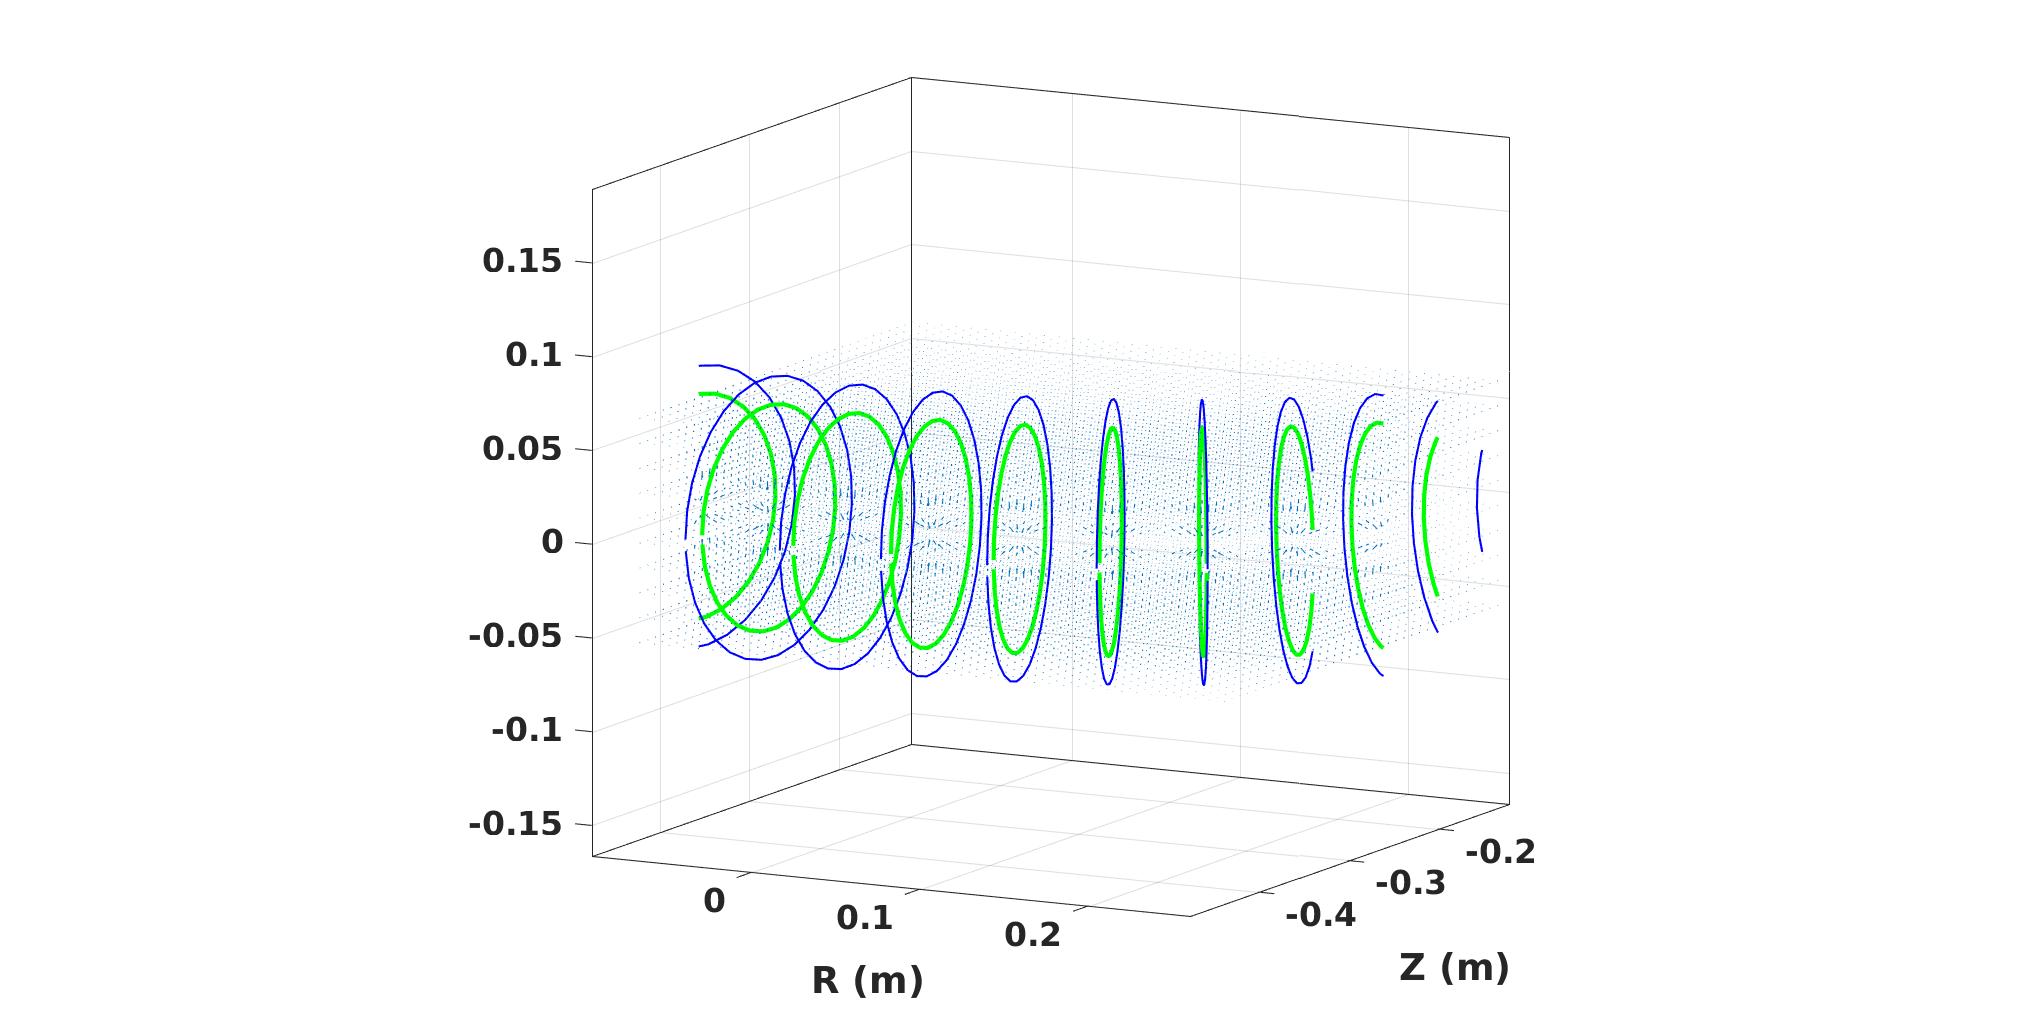
\includegraphics[scale=0.7]{../Rascunho_Resumo/tokamak.png}   
\end{figure}
\newpage
\begin{figure}[h]
\centering
\caption{Tokamak Nova-Furg, modelo feito no Blender autoria própria}
\label{fig: Rotulotokamak1}
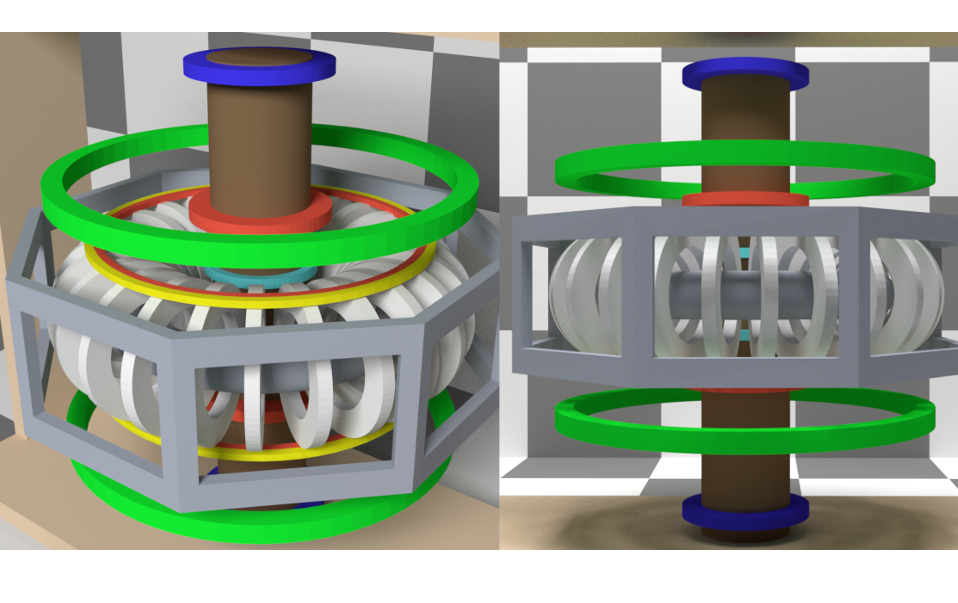
\includegraphics[scale=0.4]{tokamak12.png}    
\end{figure}

\section{Breakdown em um Tokamak}
A fase de breakdown em um tokamak é dominada por colisões entre elétrons livres e partículas neutras.
Este processo pode ser descrito pelo modelo desenvolvido por Townsend \cite{lloyd1991}. A descarga de Townsend (\textit{Townsend discharge}) é um processo de ionização de gás onde os elétrons livres, sob efeito de um campo elétrico intenso são acelerados para então colidirem com moléculas de gás e liberarem elétrons adicionais. Elétrons que também são acelerados, colidem e liberam mais elétrons adicionais. Resultando em uma multiplicação de avalanche (\textit{avalanche multiplication}) permitindo então a passagem de corrente atrávez do gás. A descarga requer uma fonte de elétrons livres e um campo elétrico intenso. O primeiro coeficiente de Townsend, explicado e modelado no apêndice \ref{Townsend}, é o número de reações de ionização por unidade de comprimento causadas por um elétron que se move paralelamente aos campos elétricos. 

\chapter{Objetivos}
O propósito principal deste trabalho é, estudar o modelo de 2 fluidos para o \textit{breakdown} no tokamak Nova-Furg. O qual é dividido em duas fazes, teórica e computacional, o objetivo teórico é obter o modelo de 2 fluidos com as devidas simplificações para seguir ao objetivo computacional onde precisa-se da distribuição de campos eletromagnéticos no tokamak, das equações relevantes linearizadas e seus respectivos solucionadores individuais implementados no Matlab.

Para finalmente, ajustar as condições de contorno e fronteira e realizar a simulação numérica que nos dará as propriedades macroscópicas do plasma. Também pretende-se obter parâmetros otimizados para o \textit{breakdown} no Nova-furg e localizar a coluna de plasma.

\chapter{Revisão Bibliográfica}
Por volta de 1950 já existia uma teoria básica para os modelos cinéticos e para os modelos MHD. Nesta mesma época os físicos soviéticos Igor Tsamm e Andrei Sakharov propuseram o conceito de tokamak. Ainda na mesma década, em 1958, Kruskal e M. D. e Kulsrud, R. M. \cite{Kruskal1958} apresentam algumas propriedades gerais de todo plasma governado pelas equações MHD, como concervação de massa, consevação de momento. Ao longo de quase duas décadas a pesquisa com o modelo de fluidos para plasmas confinados em tokamaks avança muito. Então S. P. Hirshman e S. C. Jardin (1979) \cite{hirshman} publicam  um artigo onde deduzem equações de transporte de dois fluidos. Dois anos depois é publicado por Sakanaka, P.H. (1981)\cite{Sakanaka1981} uma dedução detalhada das equações de transporte a partir dos momentos da equação de Boltzmann. Com a construção de grandes tokamaks ao redor do mundo, os modelos de fluidos são amplamente desenvolvidos para modelar o plasma nestes novos tokamaks. É usado por L. Zakharov e B. Rogers \cite{Zakharov} (1989-1993) um modelo linearizado de dois fluidos para a descrição do modo de torção interno em tokamaks. Uma abordagem computacional baseada na evolução das equações de movimento de plasma eletromagnético, não linear e de dois fluidos é usada por A Thyagaraja (2000) \cite{Thyagaraja_2000} para investigar as propriedades da turbulência e do transporte do plasma tokamak. 

Como visto anteriormente o uso do modelos de fluidos é preferível em plasmas muitos quentes e tem a vantagem de ser mais leve computacionalmente que os modelos cinéticos, como neste trabalho não iremos investigar micro efeitos no plasma e buscamos mais simplicidade, um modelo de fluidos é a melhor escolha. 
%do brackdown em tokamaks

\chapter{Cronograma}
O cronograma do trabalho encontra-se na Tabela \ref{tab-cronograma}, onde as etapas são:

\begin{enumerate}
\item Levantamento bibliográfico;
\item Análise inicial; 
\subitem Estudo do modelo de 2 fluidos para tokamak o \textit{breakdown};
\subitem Simplificações cabíveis do modelo para o Nova-Furg; 
\item Fase computacional; 
\subitem Linearizar as equações relevantes;
\subitem Inserir as equações do modelo fisico no MATLAB;
\subitem Acoplar os solucionadores individuais correspondentes a cada equação;
\subitem Definir as condições de contorno e fronteira;
\item Análise dos resultados;
\subitem Relatório/síntese dos resultados.
\end{enumerate}

\begin{table}[h!]\begin{center}
	\caption{Cronograma}\label{tab-cronograma}
	\begin{tabular*}{\textwidth}{@{\extracolsep{\fill}} c c c c c c c c c c c c}
		\toprule
		& Etapa & mar. & abr. & maio & jun. & jul. & ago. & set. & out. & nov. &\\
		\midrule
		&   1   &   x  &   x  &      &      &   x  &      &      &  x   &      &\\
		&   2   &   x  &   x  &   x  &   x  &      &      &      &      &      &\\
		&   3   &      &      &      &      &   x  &   x  &   x  &   x  &   x  &\\
		&   4   &      &      &      &      &      &      &      &   x  &   x  &\\
		\bottomrule                             
	\end{tabular*}
\end{center}\end{table}

   
\chapter{Metodologia}
Iniciaremos esta seção apresentando uma breve dedução do modelo de 2 fluidos para o \textit{breakdown}, o qual sera usado para cumprir os objetivos desta proposta. Ver lista de notações em \ref{Listanot}.
\section{Equação de Vlasov}
De acordo com o modelo de fluidos para descrever a dinâmica de um plasma consideramos que os movimentos das partículas do plasma são governados pelos campos externos aplicados mais os campos internos médios macroscópicos que são suavizados no espaço e no tempo, porcausa da presença e movimento de todas as partículas de plasma. O problema de obter os campos eletromagnéticos internos macroscópicos, no entanto, ainda é complexo e requer que uma solução auto-consistente com as equações de Maxwell e a distribuião de velocidades.
A equação de Vlasov é uma equação diferencial parcial usada para descrever a evolução temporal da função de distribuição $f_\alpha(\vv{r},\vv{v},t)$ no espaço das velocidades, posições e tempo, ou seja, descreve a evolução temporal da função de distribuição no espaço de fase. E incorpora diretamente os campos eletromagnéticos internos macroscópicos suavizados. Pode ser obtida da equação de Boltzmann na ausencia de colisões Eq. \ref{eq: boltsmam} \cite[p. 193]{bittencourt}

\begin{equation}
\label{eq: boltsmam}
\frac{\partial f_\alpha(\vv{r},\vv{v},t)}{\partial t} +\vv{v} \nabla f_\alpha(\vv{r},\vv{v},t) + a \nabla_v f_\alpha(\vv{r},\vv{v},t) = 0
\end{equation}  
onde, $\vv{v}$ é a velocidade e os operadores diferenciais $\nabla_v$ e $\nabla$ em coordenanas cartesianas são 
$$\nabla_v f_\alpha(\vv{r},\vv{v},t) =  \frac{\partial f_\alpha(\vv{r},\vv{v},t)}{\partial v_x} + \frac{\partial f_\alpha(\vv{r},\vv{v},t)}{\partial v_y} + \frac{\partial f_\alpha(\vv{r},\vv{v},t)}{\partial v_z}$$  
$$\nabla f_\alpha(\vv{r},\vv{v},t) = \frac{\partial f_\alpha(\vv{r},\vv{v},t)}{\partial x} + \frac{\partial f_\alpha(\vv{r},\vv{v},t)}{\partial y} + \frac{\partial f_\alpha(\vv{r},\vv{v},t)}{\partial z}$$
mas incluindo na Eq. \ref{eq: boltsmam} os campos suavizados internos no termo de força, obtêm-se então a Eq. \ref{eq: vlasov} que é a equação de Vlasov.
\begin{equation}
\label{eq: vlasov}
\frac{\partial f_\alpha(\vv{r},\vv{v},t)}{\partial t} +\vv{v} \nabla f_\alpha(\vv{r},\vv{v},t) + \frac{1}{m_\alpha}[\vv{F}_{ext}+q_0(\vv{E}_i+\vv{v} \times \vv{B}_i)] . \nabla_v f_\alpha(\vv{r},\vv{v},t)= 0
\end{equation}

Aqui $\vv{F}_{ext}$ representa a força externa, incluindo a força de Lorentz associada a quaisquer campos elétricos e magnéticos aplicados externamente, onde $\vv{E}_i$ e $\vv{B}_i$ são campos elétricos e magnéticos suavizados internos causados pela presença e movimento de todas as partículas carregadas dentro do plasma. Os campos eletromagnéticos macroscópicos internos $\vv{E}_i$ e $\vv{B}_i$  devem satisfazer as equações de Maxwell, uma vez que precisam ser consistentes com as densidades de carga e corrente macroscópicas existentes no próprio plasma,
\begin{equation}
\label{eq: max1}
\nabla \vv{E}_i = \frac{\rho}{\epsilon_o}
\end{equation}
\begin{equation}
\label{eq: max2}
\nabla \vv{B}_i = 0
\end{equation}
\begin{equation}
\label{eq: max3}
\nabla \times \vv{E}_i = -\frac{\partial \vv{B}_i}{\partial t}
\end{equation}
\begin{equation}
\label{eq: max4}
\nabla \times \vv{B}_i = \mu_0 (\vv{J} + \epsilon_0 \frac{\partial \vv{E}_i}{\partial t} )
\end{equation}
Onde $\mu_0 = 4\pi \times 10^{-7}$ Newtons por Ampere ao quadrado  é a permeabilidade magnética do vácuo, $\epsilon_o = \frac{1}{\mu_0 c^2}$ é constante de permissividade do vácuo com $c$ sendo a velocidade da luz no vácuo e a densidade de carga do plasma $\rho$ é dada por
\begin{equation}
\label{eq: rho}
\rho(\vv{r},t) = \sum_\alpha q_\alpha n_\alpha(\vv{r},t) = \sum_\alpha q_\alpha \int_v f_\alpha(\vv{r},\vv{v},t) d^3v
\end{equation}
E a densidade de corrente de plasma $\vv{J}$ é dada por
\begin{equation}
\label{eq: densidadecorrente}
\vv{J}(\vv{r},t) = \sum_\alpha q_\alpha n_\alpha(\vv{r},t) \vv{u}_\alpha(\vv{r},t) = \sum_\alpha  q_\alpha \int_v \vv{v} f_\alpha(\vv{r},\vv{v},t) d^3v
\end{equation}
Aqui $ \vv{u}_\alpha(\vv{r},t)$ denota a velocidade média macroscópica de cada tipo de partícula $\alpha$, ver \ref{anexo1}. As equações Eq. \ref{eq: vlasov}, Eq. \ref{eq: max1}, Eq. \ref{eq: max2}, Eq. \ref{eq: max3}, Eq. \ref{eq: max4}, Eq. \ref{eq: rho} e Eq. \ref{eq: densidadecorrente} constituem um conjunto completo de equações a serem resolvidas ao mesmo tempo. Então, por exemplo, em um procedimento iterativo assumindo valores aproximados iniciais para $\vv{E}_i(\vv{r}, t)$ e $\vv{B}_i(\vv{r}, t)$, a Eq. \ref{eq: vlasov} pode ser resolvida para produzir $f_\alpha(\vv{r},\vv{v},t)$ para os tipos diferentes de partículas. A utilização dos valores calculados em Eq. \ref{eq: rho} e Eq. \ref{eq: densidadecorrente} leva a valores para as densidades de carga e corrente $\rho$ e  $\vv{J}$ no plasma, que podem ser substituídas nas equações de Maxwell e resolvidas para $\vv{E}_i(\vv{r}, t)$ e $\vv{B}_i(\vv{r}, t)$. Esses valores são então introduzidos novamente na equação de Vlasov Eq. \ref{eq: vlasov}, e assim por diante, para obter uma solução autoconsistente para a função de distribuição de partículas individuais. Embora a equação Eq. \ref{eq: vlasov} não inclua explicitamente um termo de colisão no seu lado direito e portanto, não leve em consideração colisões de curto alcance, ela é mais geral doque parece, já que uma consideravel parte dos efeitos de interações de partículas já foram incluídas na força de Lorentz, por meio dos campos eletromagnéticos suavizados auto-consistentes internos. 

Não é necessário resolver a equação de Boltzmann para a função de distribuição, a fim de calcular as variáveis macroscópicas de interesse físico. Estas variáveis macroscópicas estão relacionadas com os momentos da função de distribuição pela equação geral de transporte, deduzina no apêndice \ref{eq: pit12}. As equações de transporte podem ser obtidas tomando os vários momentos da equação de Boltzmann. Neste trabalho sera deduzido os três primeiros momentos da equação de Boltzmann que são obtidos pela multiplicação de $m_\alpha$, $m_\alpha \vv{v}_\alpha$ e $\frac{m_\alpha \vv{v}^2_\alpha}{2}$, respectivamente, e então integrando todo o espaço de velocidade. Seguindo estas etapas, obtêm-se as equações de conservação de massa \ref{eq: pit13}, momento \ref{eq: pit23} e energia \ref{concenergia}.

\section{Equação de Conservação de Massa}

A equação de continuidade, nos garante que toda massa ganhada ou perdida no sistema é quantificada no termo $S_\alpha$.
Éssa equação pode ser obtida diretamente com a substituição na Eq. \ref{eq: pit12} do $\chi$ pela massa $m_\alpha$. Definindo a densidade de massa como $ \rho_{m\alpha} = n_\alpha m_\alpha$ temos

\begin{equation}
\label{eq: pit13}
\frac{\partial \rho_{m\alpha}}{\partial t} + \nabla \cdot (\rho_{m\alpha} \vv{u}_\alpha)  = S_\alpha 
\end{equation}

onde o termo de colisão, $S_\alpha = \left[\frac{\delta \rho_{m\alpha}}{\delta t}\right]_{coll}$, representa a taxa na qual partículas do tipo $\alpha$ são produzidas ou perdidas, por unidade de volume, como resultado de colisões.

\section{Equação de Conservação de Momento}
A equação de conservação de momento afirma que a taxa média de mudança de momento em função do tempo em cada elemento $\alpha$ do fluido, é devida às forças externas aplicadas no fluido somadas a força de pressão do próprio fluido e também domadas as forças internas devido a colisões, dispersão e produção de partículas de plasma.
Para derivar a equação de conservação de momento, substituímos na Eq. \ref{eq: pit12} o $\chi (\vv{v}_\alpha)$ pelo momento $m_\alpha \vv{v}_\alpha$ das partículas do tipo $\alpha$. 
\begin{equation}
\label{eq: p2}
\frac{\partial }{\partial t}(n_\alpha(\vv{r},t)<m_\alpha \vv{v}_\alpha>_\alpha) + \nabla \cdot (n_\alpha(\vv{r},t)<m_\alpha \vv{v}_\alpha \vv{v} >_\alpha) - n_\alpha(\vv{r},t)<\vv{a} \cdot \nabla_v m_\alpha \vv{v}_\alpha>_\alpha = 
\end{equation}

\begin{equation*}
=[\frac{\delta}{\delta t}(n_\alpha(\vv{r},t)<m_\alpha \vv{v}_\alpha>_\alpha)]
\end{equation*}
Definindo $\vv{v}_\alpha = \vv{c}_\alpha + \vv{u}_\alpha$, onde $\vv{c}_\alpha$ é a velocidade média térmica das partículas e  $\vv{u}_\alpha$ é a velocidade média de movimento toroidal. Vamos tratar de cada termo da Eq. \ref{eq: p2} semaradamente.
Aplicando a definição de valor médio \ref{anexo1} e como $ \rho_{m\alpha} = n_\alpha m_\alpha$, ficamos com $\frac{\partial }{\partial t} (n_\alpha <\chi>_\alpha)=\frac{\partial }{\partial t} (n_\alpha <m_\alpha \vv{v}_\alpha>_\alpha)$ mas $\vv{c}_\alpha$ não influencia no valor médio, então ficamos com $\frac{\partial }{\partial t} (\rho_{m\alpha} \vv{u}_\alpha)$. Aplicando a regra da cadeia na derivada parcial obtemos
\begin{equation}
\label{eq: pit14}
\frac{\partial }{\partial t} (\rho_{m\alpha} \vv{u}_\alpha) = \vv{u}_\alpha \frac{\partial \rho_{m\alpha}}{\partial t}+\rho_{m\alpha} \frac{\partial \vv{u}_\alpha}{\partial t}
\end{equation} 
Substituindo $\chi$ pelo momento $m_\alpha \vv{v}_\alpha$ temos $\nabla \cdot (n_\alpha <\chi \vv{v}>_\alpha) =  \nabla \cdot (n_\alpha <m_\alpha \vv{v}_\alpha \vv{v}>_\alpha)$ e tirando $m_\alpha$ para fora da média, pois é constante temos $\nabla \cdot (n_\alpha m_\alpha < \vv{v} \cdot \vv{v}>_\alpha)$ nota-se que dentro do termo de média $ \vv{v}_\alpha$ é igual $\vv{v}$ pois o tipo de partícula $\alpha$ já esta representado na operação valor médio $< >_\alpha$ ficamos com $\nabla \cdot (\rho_{m\alpha} <\vv{v} \cdot \vv{v}>)$.  Aplicando a definição de valor médio \ref{anexo1} obtemos 
\begin{equation}
\label{eq: pit15}
\nabla \cdot (\rho_{m\alpha} <\vv{v} \cdot \vv{v}>) = \nabla \cdot ( \rho_{m\alpha}\vv{u}_\alpha \cdot \vv{u}_\alpha + \rho_{m\alpha}<\vv{c}_\alpha \cdot \vv{c}_\alpha>)
\end{equation} 
já que $\vv{c} \cdot \vv{u} = 0$ pois $\vv{c}$ vai em todas as direções então não contribui com a velocidade, e o valor médio de $\vv{v}_\alpha$ é por definição igual a $\vv{u}_\alpha$.
No termo seguinte, $n_\alpha(\vv{r},t)<\vv{a} \cdot \nabla_v m_\alpha \vv{v}>_\alpha$ rearanjamos os termos ficando com $n_\alpha(\vv{r},t)<(m_\alpha \vv{a} \cdot \nabla_v) \vv{v}>_\alpha$ observando que massa vezes aceleração é força, $\vv{F} = \vv{a} \cdot m_\alpha $, temos $n_\alpha(\vv{r},t) <(\vv{F} \cdot \nabla_v)\vv{v}>_\alpha$ que nos da
\begin{equation}
\label{eq: pit16}
n_\alpha(\vv{r},t) <(\vv{F} \cdot \nabla_v)\vv{v}>_\alpha=n_\alpha(\vv{r},t)<\vv{F}>_\alpha
\end{equation}
pois $(\vv{F} \cdot \nabla_v)\vv{v} = \vv{F} \cdot (\nabla_v\vv{v})$ e $\nabla_v\vv{v} = 1$. Definindo $R_\alpha$ igual a taxa de mudança de momento devido ao espalhamento onde
\begin{equation}
\label{eq: pit17}
R_\alpha = \left[\frac{\delta}{\delta t}(n_\alpha(\vv{r},t)<m_\alpha \vv{v}_\alpha>_\alpha)\right]=\left[\frac{\delta}{\delta t}(\rho_{m\alpha}\vv{u}_\alpha)\right]
\end{equation}
e  $\mathcal{R}_\alpha$ igual a taxa de mudança de momento devido à produção de partículas de plasma onde
\begin{equation}
\label{eq: pit18}
\mathcal{R}_\alpha = \left[\frac{\delta}{\delta t}(n_\alpha(\vv{r},t)<m_\alpha \vv{v}_\alpha>_\alpha)\right] = \left[\frac{\delta}{\delta t}(\rho_{m\alpha}\vv{u}_\alpha)\right]
\end{equation}
Substituindo Eq. \ref{eq: pit14}, Eq. \ref{eq: pit15}, Eq. \ref{eq: pit16}, Eq. \ref{eq: pit17}, Eq. \ref{eq: pit18} em Eq. \ref{eq: p2} obtemos
\begin{equation}
\label{eq: pit19}
\vv{u}_\alpha \frac{\partial \rho_{m\alpha}}{\partial t} + \rho_{m\alpha} \frac{\partial \vv{u}_\alpha}{\partial t}+ \nabla \cdot (\rho_{m\alpha} \vv{u}_\alpha \vv{u}_\alpha)+
\end{equation} 
\begin{equation*}
+\nabla \cdot (\rho_{m\alpha} <\vv{c}_\alpha \cdot \vv{c}_\alpha>)-n_\alpha<\vv{F}>_\alpha=R_\alpha + \mathcal{R}_\alpha
\end{equation*}
Definindo o tensor $\mathbb{P}_\alpha=\rho_{m\alpha} <\vv{c}_\alpha \cdot \vv{c}_\alpha>$ que representa a força por unidade de volume dentro do plasma devido aos movimentos aleatórios das partículas. Temos
\begin{equation}
\label{eq: pit20}
\nabla \cdot (\rho_{m\alpha} \vv{u}_\alpha \vv{u}_\alpha) =  \rho_{m\alpha}(\vv{u}_\alpha \cdot \nabla)\vv{u}_\alpha + [\nabla \cdot (\rho_{m\alpha} \vv{u}_\alpha)]\vv{u}_\alpha
\end{equation}
Fazendo força média igual a força de Lorentz temos 
\begin{equation}
\label{eq: pit20.1}
<\vv{F}>_\alpha = q_\alpha (\vv{E} + \vv{u}_\alpha \times \vv{B})
\end{equation} e substituindo as Eq. \ref{eq: pit20} e Eq. \ref{eq: pit20.1} em Eq. \ref{eq: pit19} teremos
\begin{equation}
\label{eq: pit21}
 \vv{u}_\alpha \frac{\partial \rho_{m\alpha}}{\partial t} + \rho_{m\alpha} \frac{\partial \vv{u}_\alpha}{\partial t}+ \rho_{m\alpha} (\vv{u}_\alpha \cdot \nabla)\vv{u}_\alpha+[\nabla \cdot (\rho_{m\alpha} \vv{u}_\alpha)]\vv{u}_\alpha  =
\end{equation}
\begin{equation*}
n_\alpha q_\alpha (\vv{E} + \vv{u}_\alpha \times \vv{B})-\nabla \cdot \mathbb{P}_\alpha + R_\alpha + \mathcal{R}_\alpha
\end{equation*}
rearanjando
\begin{equation}
\label{eq: pit22}
\rho_{m\alpha} \left[\frac{\partial \vv{u}_\alpha}{\partial t} + (\vv{u} \cdot \nabla)\vv{u}_\alpha \right]+ \vv{u}_\alpha \left[ \frac{\partial \rho_{m\alpha}}{\partial t} + \nabla \cdot (\rho_{m\alpha} \vv{u}_\alpha)  \right] = R_\alpha + \mathcal{R}_\alpha +n_\alpha(\vv{r},t) q_\alpha (\vv{E} + \vv{u}_\alpha \times \vv{B})-\nabla \cdot \mathbb{P}_\alpha 
\end{equation}
No entanto, o segundo termo no lado esquerdo da Eq. \ref{eq: pit22} é a equação de conservação de massa Eq. \ref{eq: pit13} então se não considerarmos as colisões que levam à geração ou perda de partículas, ou seja $S_\alpha = 0$, podemos simplificar a equação para
\begin{equation}
\label{eq: pit23}
\rho_{m\alpha} \left[\frac{\partial \vv{u}_\alpha}{\partial t} + (\vv{u} \cdot \nabla)\vv{u}_\alpha \right] =  R_\alpha + \mathcal{R}_\alpha +n_\alpha(\vv{r},t) q_\alpha (\vv{E} + \vv{u}_\alpha \times \vv{B})-\nabla \cdot \mathbb{P}_\alpha 
\end{equation}
A equação de concervação de momento estabelece a condição necessária para garantir a conservação do momento do sistema. O termo $-\nabla \cdot \mathbb{P}_\alpha $ representa a força causada pelas variações aleatórias nas velocidades de cada partícula que é exercida em um volume unitário do plasma. Esta força em cada unidade de volume também inclui forças associadas à pressão escalar e forças de corte tangenciais, que são as forças viscosas. No nosso  caso, o efeito da viscosidade é pequeno não sendo importante no nosso plasma. Os termos não-diagonais de $\mathbb{P}_\alpha$ podem ser desprezados.  Além disso, no caso em que quando a distribuição de velocidades de cada tipo de partícula é isotrópica (não à direção privilegiada, suas propriedades são as mesmas em qualquer direção). Os termos diagonais de $\mathbb{P}_\alpha$ são todos iguais e representam a pressão cinética escalar $p_\alpha$. Assim, desconsiderando os efeitos de viscosidade e considerando uma distribuição de velocidade isotrópica, temos $\mathbb{P}_\alpha = p_\alpha$, e a força por unidade de volume se torna $-\nabla \cdot \mathbb{P}_\alpha = -\nabla p_\alpha$, de acordo com a \cite[Cap 6]{bittencourt}.


\section{Equação de Conservação de Energia}
A equação de conservação de energia nos garante que toda energia cinética ganha ou perdida no sistema veio de colisões com outras partículas do sistema ou foi causado pelo campo elétrico $\vv{E}$.
Para derivar a equação de conservação de energia, substituímos  na Eq. \ref{eq: pit12} o $\chi (\vv{v}_\alpha)$ pela energia cinética $\frac{m_\alpha \vv{v}^2_\alpha}{2}$ das partículas do tipo $\alpha$ obtendo
\begin{equation}
\label{eq: p3}
\frac{\partial }{\partial t}(n_\alpha(\vv{r},t)<\frac{1}{2}m_\alpha v_{\alpha}^2>_\alpha) + \nabla \cdot (n_\alpha(\vv{r},t)<\frac{1}{2}m_\alpha v_{\alpha}^2 \vv{v} >_\alpha) - n_\alpha(\vv{r},t)<\vv{a} \cdot \nabla_v \frac{1}{2}m_\alpha v_{\alpha}^2>_\alpha = 
\end{equation}
\begin{equation*}
=[\frac{\delta}{\delta t}(n_\alpha(\vv{r},t)<\frac{1}{2}m_\alpha v_{\alpha}^2>_\alpha)]
\end{equation*}
O primeiro termo da Eq. \ref{eq: p3} sera simplificado trocando $ n_\alpha(\vv{r},t) m_\alpha$ por $\rho_{m\alpha}$ 
\begin{equation}
\label{eq: pit24}
\frac{\partial }{\partial t}(n_\alpha<\frac{m_\alpha \vv{v}^2_\alpha}{2}>_\alpha)=\frac{\partial }{\partial t}(\frac{\rho_{m\alpha}}{2}<\vv{v}^2_\alpha>_\alpha)
\end{equation}
abrindo $\vv{v}^2_\alpha$ a Eq. \ref{eq: pit24} fica
\begin{equation}
\label{eq: pit24.1}
\frac{\partial }{\partial t}(\frac{\rho_{m\alpha}}{2}<\vv{v}^2>_\alpha)=\frac{\partial }{\partial t}(\frac{\rho_{m\alpha}}{2}(\vv{u}_\alpha \cdot \vv{u}_\alpha) + \frac{\rho_{m\alpha}}{2}<\vv{c}_\alpha \cdot \vv{c}_\alpha>_\alpha)
\end{equation} 
Como a velocidade aleatória não tem sentido privelegiado, temos para qualquer partícula $|\vv{v}^2| = v_x^2 + v_y^2 + v_z^2$ e como são muitas partículas que se movem em direções aleatórias, os valores médios dos quadrados das componentes de suas velocidades são iguais, logo, $v_x^2 = \frac{1}{3} |\vv{v}^2|$ então da teoria cinética dos gases obtemos $p=\frac{nMv_x^2}{V}$ onde $M$ é a massa molar do gás de origem do plasma, $p$ é a pressão e $n$ o numero de moles. No nosso caso $\frac{nMv_x^2}{V} = \frac{nM <c^2_\alpha>}{3V} $ e a densidade de massa $ \rho_{m\alpha} = n_\alpha m_\alpha$ pode subtituir $\frac{nM}{V}$ nos deixando com $\rho_{m\alpha}<c^2_\alpha>=3p_\alpha$. 
Então a Eq. \ref{eq: pit24.1} simplifica para 
\begin{equation}
\label{eq: pit24.12}
\frac{\partial }{\partial t}(\frac{\rho_{m\alpha}}{2}(\vv{u}_\alpha \cdot \vv{u}_\alpha) + \frac{\rho_{m\alpha}}{2}<\vv{c}_\alpha \cdot \vv{c}_\alpha>_\alpha)=\frac{\partial }{\partial t}  \left( \frac{1}{2} 3p_\alpha+\frac{1}{2} \rho_{m\alpha}\vv{u}^2_\alpha \right) 
\end{equation} 
O segundo termo da Eq.\ref{eq: p3} pode ser organizado rearanjando termos e trocando $ n_\alpha(\vv{r},t) m_\alpha$ por $\rho_{m\alpha}$ que fica
\begin{equation}
\label{eq: pit24.10}
\nabla \cdot (n_\alpha(\vv{r},t)<\frac{1}{2}m_\alpha v_{\alpha}^2 \vv{v} >_\alpha) = \nabla \cdot \left[ \frac{\rho_{m\alpha}}{2}<(\vv{v} \cdot \vv{v})\vv{v}>_\alpha \right]
\end{equation}
Lembrando que $\vv{v} = \vv{u}_\alpha + \vv{c}_\alpha$ então  $<(\vv{v} \cdot \vv{v})\vv{v}>_\alpha$ pode ser expandido da seguinte maneira $
<[(\vv{u}_\alpha + \vv{c}_\alpha) \cdot (\vv{u}_\alpha + \vv{c}_\alpha)](\vv{u}_\alpha + \vv{c}_\alpha)> = <(\vv{u}^2_\alpha + \vv{c}^2_\alpha+2\vv{u}_\alpha \cdot \vv{c}_\alpha)(\vv{u}_\alpha + \vv{c}_\alpha)>$. Pode-se escrever a equação de conservação de energia de outra forma se substituir o fluxo de calor e o tensor de pressão cinética definidos como
\begin{equation}
\mathbb{P}_\alpha = \rho_{m\alpha}<\vv{c}_\alpha \cdot \vv{c}_\alpha> 
\end{equation}
onde $\mathbb{P}_\alpha$ é o tensor de pressão cinética
\begin{equation}
\vv{q}_\alpha = \frac{1}{2} \rho_{m\alpha} <c^2_\alpha  \vv{c}_\alpha>
\end{equation}
onde $\vv{q}_\alpha$ é o fluxo de calor
mas como vimos a pressão cinética é dada por $\rho_{m\alpha}<|\vv{c}^2|_\alpha>=3p_\alpha$ então a Eq. \ref{eq: pit24.10} fica
\begin{equation}
\label{eq: pit24.11}
\nabla \cdot \left[ \frac{\rho_{m\alpha}}{2}<(\vv{v} \cdot \vv{v})\vv{v}>_\alpha \right]= \nabla \cdot \left[ \frac{\rho_{m\alpha}}{2}\vv{u}_\alpha+\frac{1}{2}(3p_\alpha) + \mathbb{P}_\alpha \cdot \vv{u}_\alpha + \vv{q}_\alpha \right]
\end{equation}
simplificando \ref{eq: pit24.11} obtemos
\begin{equation}
\label{eq: pit24.13}
\nabla \cdot \left[ \frac{\rho_{m\alpha}}{2}\vv{u}_\alpha+\frac{1}{2}(3p_\alpha) + \mathbb{P}_\alpha \cdot \vv{u}_\alpha + \vv{q}_\alpha \right] = 
\end{equation} 

\begin{equation*}
\nabla \cdot \left[ \frac{1}{2}\rho_{m\alpha}|\vv{u}|^2_\alpha \vv{u}_\alpha) \right]+ \frac{3}{2}p_\alpha (\nabla \cdot \vv{u}_\alpha) +  \frac{1}{2}(\vv{u}_\alpha \cdot \nabla)(3p_\alpha)+\nabla \cdot (\mathbb{P} \cdot \vv{u}_\alpha) + \nabla \cdot \vv{q}_\alpha
\end{equation*}
Para o terceiro termo substituimos $\vv{a} =  \frac{\vv{F}}{m_\alpha}$ 
\begin{equation}
\label{eq: pit24.21}
n_\alpha(\vv{r},t) <\vv{a} \cdot \nabla_v \frac{m_\alpha \vv{v}^2_\alpha}{2}>_\alpha = n_\alpha(\vv{r},t)<\frac{\vv{F}}{m_\alpha} \cdot \nabla_v \left( \frac{m_\alpha \vv{v}^2}{2}\right)>_\alpha 
\end{equation}
resolvendo $\nabla_v ( \frac{m_\alpha \vv{v}^2}{2})$ obtemos $\frac{2m_\alpha \vv{v}}{2}$ e subtituindo em \ref{eq: pit24.2} e cancelando o $2m_\alpha$ que esta no denominador e dividendo ficamos com
\begin{equation}
\label{eq: pit24.4}
n_\alpha(\vv{r},t)<\frac{\vv{F}}{m_\alpha} \cdot \nabla_v \left( \frac{m_\alpha \vv{v}^2}{2}\right)>_\alpha = n_\alpha(\vv{r},t) <\vv{F} \cdot \vv{v}>_\alpha
\end{equation}
Substituindo as quantidades Eq. \ref{eq: pit24.12}, Eq. \ref{eq: pit24.13} e Eq. \ref{eq: pit24.4} na Eq. \ref{eq: p3} temos
\begin{equation}
\label{eq: p4}
\frac{\partial }{\partial t}  \left( \frac{1}{2} 3p_\alpha+\frac{1}{2} \rho_{m\alpha}\vv{u}^2_\alpha \right) +\nabla \cdot \left[ \frac{1}{2}\rho_{m\alpha}|\vv{u}|^2_\alpha \vv{u}_\alpha) \right]+ \frac{3}{2}p_\alpha (\nabla \cdot \vv{u}_\alpha) +  \frac{1}{2}(\vv{u}_\alpha \cdot \nabla)(3p_\alpha)+ 
\end{equation}
\begin{equation*}
\nabla \cdot (\mathbb{P} \cdot \vv{u}_\alpha) + \nabla \cdot \vv{q}_\alpha-n_\alpha(\vv{r},t) <\vv{F} \cdot \vv{v}>_\alpha =[\frac{\delta}{\delta t}(n_\alpha(\vv{r},t)<\frac{1}{2}m_\alpha v_{\alpha}^2>_\alpha)]
\end{equation*}

Definindo $M_\alpha$ que representa a taxa de mudança de densidade de energia devido a colisões
\begin{equation}
M_\alpha = \frac{3}{2} \left(  \frac{\partial p_\alpha}{\partial t}  \right) + \frac{\partial}{\partial t} \left[ \frac{1}{2}\rho_{m\alpha}|\vv{u}|^2_\alpha \right]+ \nabla \cdot \left[\frac{1}{2}\rho_{m\alpha}<(\vv{v} \cdot \vv{v})\vv{v}>_\alpha \right] -  n_\alpha(\vv{r},t)<\vv{F} \cdot \vv{v}>_\alpha
\end{equation}

Usando $\frac{D}{Dt} = \frac{\partial }{\partial t} + \vv{u}_\alpha \cdot \nabla$ que é a derivada total do tempo obtemos

\begin{equation}
\label{eq: p5.1}
\frac{D}{Dt} \left( \frac{3}{2}p_\alpha \right) + \left(\frac{3}{2}p_\alpha \right)  \nabla \cdot \vv{u}_\alpha +  \frac{\partial }{\partial t} \left(\frac{\rho_{m\alpha}}{2} |\vv{u}|^2_\alpha \right) +\nabla \cdot \left[ \frac{1}{2}\rho_{m\alpha}|\vv{u}|^2_\alpha \vv{u}_\alpha \right] = 
\end{equation}
\begin{equation*}
\nabla \cdot (\mathbb{P} \cdot \vv{u}_\alpha) + \nabla \cdot \vv{q}_\alpha-n_\alpha(\vv{r},t) <\vv{F} \cdot \vv{v}>_\alpha = M_\alpha
\end{equation*}
Reescrevendo os termos $\frac{\partial }{\partial t} \left(\frac{\rho_{m\alpha}}{2} |\vv{u}|^2_\alpha \right) +\nabla \cdot \left[ \frac{1}{2}\rho_{m\alpha}|\vv{u}|^2_\alpha \vv{u}_ \alpha \right]$ em função da derivada total $\frac{D}{Dt}$ ficamos com
\begin{equation}
\frac{\partial }{\partial t} \left(\frac{\rho_{m\alpha}}{2}\vv{u}_\alpha \cdot \vv{u}_\alpha \right) +\nabla \cdot \left[ \frac{1}{2}\rho_{m\alpha}(\vv{u}_\alpha \cdot \vv{u}_ \alpha) \vv{u}_\alpha \right] = 
\end{equation}

\begin{equation*}
= \frac{1}{2}|\vv{u}|^2_\alpha \frac{\partial \rho_{m\alpha} }{\partial t} + \rho_{m\alpha} \vv{u}_\alpha \cdot \frac{\partial \vv{u}_\alpha}{\partial t} +
\frac{1}{2}|\vv{u}|^2_\alpha \nabla \cdot \left[ \rho_{m\alpha}  \vv{u}_\alpha \right] + \rho_{m\alpha}  \vv{u}_\alpha  \cdot \left[ (\vv{u}_\alpha \cdot \nabla )\vv{u}_\alpha  \right] = 
\end{equation*}

\begin{equation*}
= \frac{1}{2}|\vv{u}|^2_\alpha \left[  \frac{\partial \rho_{m\alpha} }{\partial t} +  \nabla \cdot (\rho_{m\alpha} \vv{u}_\alpha)   \right] + \rho_{m\alpha}  \vv{u}_\alpha \cdot \frac{\partial \vv{u}_\alpha}{\partial t}
\end{equation*}
 Usando as equações de concervação de massa e momento, Eq. \ref{eq: pit13} e Eq. \ref{eq: pit23} 
\begin{equation}
\label{eq: p6}
 \frac{1}{2}|\vv{u}|^2_\alpha S_\alpha + n_\alpha(\vv{r},t)\vv{u}_\alpha<F>_\alpha-\vv{u}_\alpha \cdot (\nabla \cdot \mathbb{P})-|\vv{u}|^2_\alpha S_\alpha
 \end{equation} 
 Substituindo em Eq.  \ref{eq: p6} o resultado de Eq. \ref{eq: p5.1}
 \begin{equation}
\label{eq: p5}
\frac{D}{Dt} \left( \frac{3}{2}p_\alpha \right) + \left(\frac{3}{2}p_\alpha \right)  \nabla \cdot \vv{u}_\alpha +  \frac{\partial }{\partial t} \left(\frac{\rho_{m\alpha}}{2} |\vv{u}|^2_\alpha \right) +\nabla \cdot \left[ \frac{1}{2}\rho_{m\alpha}|\vv{u}|^2_\alpha \vv{u}_\alpha \right]+  = 
\end{equation}
\begin{equation*}
\nabla \cdot (\mathbb{P} \cdot \vv{u}_\alpha) + \nabla \cdot \vv{q}_\alpha-n_\alpha(\vv{r},t) <\vv{F} \cdot \vv{v}>_\alpha = M_\alpha
\end{equation*}
Definindo  $Q_\alpha$ como sendo a taxa de variação da densidade de energia devido ao espalhamento onde
\begin{equation}
Q_\alpha = \left[ \frac{\delta}{\delta t}(n_\alpha<\frac{m_\alpha \vv{v}^2_\alpha}{2}>_\alpha) \right] = \left[ \frac{\delta}{\delta t}\left( \frac{1}{2} \rho_{m\alpha} u^2_\alpha \right) \right]
\end{equation}
E definindo $\mathcal{E}_\alpha$ que representa a taxa de variação da densidade de energia devido a produção de partículas de plasma onde 
\begin{equation}
\mathcal{E}_\alpha = \left[ \frac{\delta}{\delta t}(n_\alpha<\frac{m_\alpha \vv{v}^2_\alpha}{2}>_\alpha) \right] = \left[ \frac{\delta}{\delta t}\left( \frac{1}{2} \rho_{m\alpha} u^2_\alpha \right) \right]
\end{equation}
Desta forma a Eq. \ref{eq: p4} torna-se então
\begin{equation}
\label{concenergia}
\frac{3}{2} \left( \frac{\partial p_\alpha}{\partial t} + \vv{u}_\alpha \cdot \nabla p_\alpha\right)+ \frac{3}{2} p_\alpha (\nabla \cdot \vv{u}_\alpha)+(\mathbb{P}_\alpha \cdot \nabla)\cdot \vv{u}_\alpha + \nabla \cdot \vv{q}_\alpha =  
\end{equation}
\begin{equation*}
= Q_\alpha + \mathcal{E}_\alpha-\vv{u}_\alpha \cdot \vv{R}_\alpha - \vv{u}_\alpha \cdot \mathcal{R}_\alpha+\frac{1}{2}u^2_\alpha S_\alpha
\end{equation*}

\section{Simplificações}
 Assumindo $n_e = n_i = n_0$ onde $n_0$ é a densidade eletronica em $t = 0$, $n_e$ é a densidade numérica elétrons e $n_i$ é a densidade numérica de íons. Para modelar o Breakdown do plasma no tokamak Nova-Furg, usando um modelo de dois fluidos. Assumiremos que o plasma é composto por um fluido de elétrons e um único fluido ionizado, ambos sendo incompressíveis, $\nabla \vv{u}_{\alpha} = 0$,  um fluido ideal que não possua viscosidade $\mathbb{P}_{\alpha} = p_{\alpha}$, quase neutro $n_e = n_i = n$, e adiabático $\nabla \vv{q}_{\alpha} = 0$, ou seja, com escalas de tempo suficientemente curtas para que não haja difusão de calor, portanto o processo sera considerdo adiabático e o transporte de energia é predominantemente convectivo. Para melhorar a estabilidade numérica, vamos considerar o fluxo total de partículas a ser composto por um termo convectivo e difusivo, isto é, $\Gamma=n\vv{u}_{\alpha}-D_{\alpha} \nabla n$ com $D_e = D_i = D$ sendo o coeficiente de difusão de partículas. Além do mais, adimitimos também que o gás neutro esteja em repouso e à temperatura ambiente. Portanto, os termos de momento e fonte de energia devido à produção de partículas de plasma $\mathcal{R}_{\alpha}$ e $\mathcal{E}_{\alpha}$ ficam sem contribuir para o momento e temperatura do plasma. Com essas suposições,
o conjunto de equações consideradas neste modelo são:

\begin{equation}
\frac{\partial n}{\partial t} + \nabla \cdot (n \vv{u}_\alpha) = \frac{S_\alpha}{m_\alpha}+D\nabla^2 n
\end{equation}
\begin{equation}
m_\alpha n \left[ \frac{\partial \vv{u}_\alpha}{\partial t} + (\vv{u}_\alpha \cdot \nabla)\vv{u}_\alpha \right] =  q_\alpha n (\vv{E}+\vv{u}_\alpha \times \vv{B}) - \nabla p_\alpha + \vv{R}_\alpha - \vv{u}_\alpha S_\alpha 
\end{equation}
\begin{equation} 
\frac{3}{2} \left( \frac{\partial p_\alpha}{\partial t} + \vv{u}_\alpha \cdot \nabla p_\alpha \right) =Q_\alpha -\vv{u}_\alpha \cdot \vv{R}_\alpha \frac{1}{2} u^2_\alpha S_\alpha
\end{equation}
Aqui, vamos supor que o termo de troca de momento $\vv{R}_\alpha$ pode ser modelado por
\begin{equation}
\vv{R}_\alpha = m_\alpha n \sum_\rho  \mu_{\alpha \rho}(\vv{u}_\alpha - \vv{u}_\rho)
\end{equation}
e portanto,
\begin{equation}
\vv{R}_e = m_e n \nu_{en}\vv{u}_e+ne\eta \vv{J}
\end{equation}
\begin{equation}
\vv{R}_i = m_i n \nu_{in}\vv{u}_i+ne\eta \vv{J}
\end{equation}
com $\eta$ sendo a resistividade paralela do Spitzer \cite[2.16]{tokamaks}, e que os termos de troca de elétrons e de íons podem ser modelados por
\begin{equation}
\vv{Q}_e = -\vv{Q}_i = -\frac{3ne^2}{m_i} \eta (p_e-p_i)
\end{equation}
\\
O conjunto final de equações que devem ser resolvidas é então\\
equações de conservação de massa
\begin{equation}
\label{eq: pit1}
\frac{\partial n}{\partial t} + \nabla.(n \vv{u}_e) = \frac{S_e}{m_e}+D\nabla^2 n
\end{equation}
\begin{equation} 
\label{eq: pit2}
\frac{\partial n}{\partial t} + \nabla.(n \vv{u}_i) = \frac{S_i}{m_i}+D\nabla^2 n
\end{equation}
equações de conservação de momento
%eletron
\begin{equation}
\label{eq: pit51}
[\frac{\partial \vv{u}_e}{\partial t} + (\vv{u}_e . \nabla)\vv{u}_e] = - \frac{e}{m_e} (\vv{E}+\vv{u}_e \times \vv{B}) - \frac{\nabla p_e}{m_e n} - (\nu_{en}+\frac{S_e}{m_e n})\vv{u}_e + \frac{e}{m_e}\eta \vv{J} 
\end{equation}
%ion
\begin{equation}
[\frac{\partial \vv{u}_i}{\partial t} + (\vv{u}_i . \nabla)\vv{u}_i] = - \frac{e}{m_i} (\vv{E}+\vv{u}_i \times \vv{B}) - \frac{\nabla p_i}{m_i n} - (\nu_{in}+\frac{S_i}{m_i n})\vv{u}_i + \frac{e}{m_i}\eta \vv{J} 
\end{equation}
equações de energia do eletron
\begin{equation}
\frac{3}{2} (\frac{\partial p_e}{\partial t} + \vv{u}_e . \nabla p_e) = -\frac{3ne^2}{m_i} \eta(p_e-p_i)-ne\eta \vv{u}_e.\vv{J}+(2 \nu_{en} + \frac{S_e}{m_e n} )\frac{1}{2}m_en{u_e}^2
\end{equation}

\begin{equation}
\frac{3}{2} (\frac{\partial p_i}{\partial t} + \vv{u}_i . \nabla p_i) = -\frac{3ne^2}{m_i} \eta(p_e-p_i)-ne\eta \vv{u}_i.\vv{J}+(2 \nu_{in} + \frac{S_i}{m_i n} )\frac{1}{2}m_in{u_i}^2
\end{equation}

Suponhamos agora que, durante a fase inicial, os íons podem ser considerados em repouso ($\vv{u}_i = 0$) e, portanto, podemos remover a equação de conservação do momento iônico. Vamos também adicionar as equações Eq. \ref{eq: pit1} e Eq. \ref{eq: pit2}. Para isso, teremos que definir um termo de fonte de partículas que explique o número de partículas em si em vez da massa de partículas: $\zeta_\alpha = S_\alpha / m_\alpha$. Note que para um plasma ionizado sozinho, podemos dizer que $\zeta_e = \zeta_i = \zeta = n(\nu_{ion} - \nu_{loss})$. Também assumiremos que $\nu_{ion} = \alpha_T u_e = \alpha_T J / (ne)$ e $v_{loss} = u_{e, ||} / L_{eff} = \vv{J}.\vv{B} (Bne)$. Aqui, $\alpha_T$ é o primeiro coeficiente de Townsend \ref{Townsend}. Com todas essas suposições, o conjunto de equações simplifica para
\begin{equation}
\frac{\partial n}{\partial t} = \nu_{ion} - \nu_{loss}+D\nabla^2n
\end{equation}

\begin{equation}
m_e[\frac{\partial \vv{u}_e}{\partial t} + (\vv{u}_e . \nabla)\vv{u}_e] = - e (\vv{E}+\vv{u}_e \times \vv{B}) - \frac{\nabla p_e}{n} -(\nu_{en}+\nu_{ion}-\nu_{loss})m_e \vv{u}_e+ e\eta \vv{J} 
\end{equation}

\begin{equation}
\frac{3}{2} (\frac{\partial p_e}{\partial t} + \vv{u}_e . \nabla p_e) = -\frac{3ne^2}{m_i} \eta(p_e-p_i)-ne\eta \vv{u}_e.\vv{J}+(2 \nu_{en} + \nu_{ion} - \nu_{loss} )\frac{1}{2}m_en{u_e}^2
\end{equation}

\begin{equation}
\frac{\partial p_i}{\partial t} = \frac{2ne^2}{m_i}\eta(p_e-p_i)
\end{equation}
Vamos agora reescrever este conjunto de equações em termos da densidade de corrente
\begin{equation}
\frac{\partial n}{\partial t} = \nu_{ion} - \nu_{loss}+D\nabla^2n
\end{equation}

\begin{equation}
\frac{\partial \vv{J}}{\partial t} =  \frac{ne^2}{m_e} \vv{E} -\vv{J}(\nu_{in}+\nu_{en}+\nu_{ion}-\nu_{loss}) -\frac{e}{m_e}\vv{J} \times \vv{B}+\frac{e}{m_e}\nabla p_e 
\end{equation}

\begin{equation}
\frac{\partial p_e}{\partial t} = \frac{3}{2}(1+\frac{2 \nu_{en} + \nu_{ion} - \nu_{loss}}{2\nu_{ei}})\eta J^2  -\frac{2ne^2}{m_i} \eta (p_e-p_i)
\end{equation}

\begin{equation}
\frac{\partial p_i}{\partial t} = \frac{2ne^2}{m_i}\eta(p_e-p_i)
\end{equation}

\chapter{Sistema de Coordenadas Pseudotoridais}
Faremos uma mudança de coordenadas, para um sistema de coordenadas que chamaremos de pseudotoridal, é um sistema composto por coordenadas cílindricas que se fecham em si mesmas, explicando de outra forma, é como se no interior de um toróide (com as dimenções internas da câmera de vácuo do tokamak Nova-Furg), cada seção reta circular fosse graduada com um sistema de coordenadas polares ($R,\theta$) e com um angulo $\phi$ que representa o quanto a seção reta do toróide se deslocou da origem onde $\phi=0$ ver figuras \ref{fig: btokamak5} e \ref{fig: btokamak6}. Após sera feito a adptação do modelo de dois fluidos para as coordenadas ($r,\theta,\phi$).
\newpage
\begin{figure}[H]
\centering
\caption{Coordenadas Pseudotoridais}
\label{fig: btokamak5}
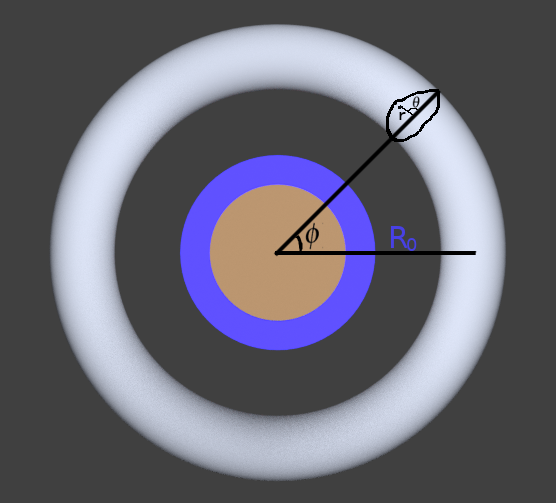
\includegraphics[scale=0.7]{pseudotoridal1.png}
\caption{O ponto $A$ representado em coordenadas pseudotoridais} 
\label{fig: btokamak6}
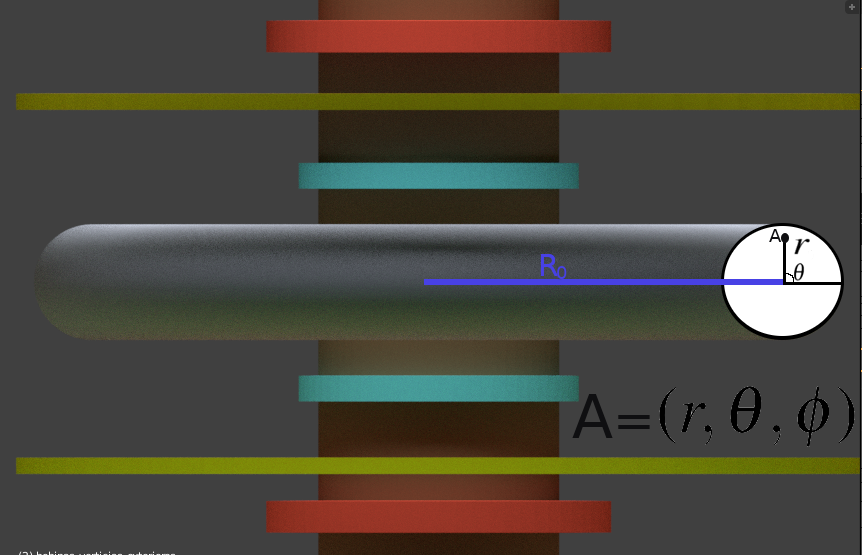
\includegraphics[scale=0.45]{pseudotoridal2.png}    
\end{figure}

O sistema de coordenadas usado no modelo de 2 fluidos deduzido neste trabalho é o sistema ($R,Z',\phi$). A regra para mudar do sistema pseudotoridal ($r,\theta,\phi$) para o sistema do modelo ($R,Z',\phi$) é
\begin{equation}
 R = R_D+r \cos(\theta)
\end{equation}
\begin{equation}
 Z' = r \sin(\theta)
 \end{equation}
A terceira coordenada $\phi$ permanece a mesma. As funções $X_s(R,Z',\phi)$, $Y_s(R,Z',\phi)$ e $Z_s(R,Z',\phi)$ usadas para mudar das coordenadas ($R,Z',\phi$) para as coordenadas cartesianas ($X,Y,Z$) são obtidas facilmente projetando o $R$ na direção de $X$ e depois na direção de $Y$.
\begin{equation}
X_s(R,Z',\phi) = R \cos(\phi)
\end{equation}
\begin{equation}
Y_s(R,Z',\phi) = R \sin(\phi)
\end{equation}
\begin{equation}
Z_s(R,Z',\phi) = Z'
\end{equation}
Substituindo $R$ e $Z'$ obtemos então as funções $X(r,\theta,\phi)$, $Y(r,\theta,\phi)$ e $Z(r,\theta,\phi)$ que são a regra para mudar de coordenadas pseudotoridais para coordenadas cartesianas.
\begin{equation}
\label{rX}
X(r,\theta,\phi) = (R_D+r \cos(\theta)) \cos(\phi)
\end{equation}
\begin{equation}
\label{rY}
Y(r,\theta,\phi) = (R_D+r \cos(\theta)) \sin(\phi)
\end{equation}
\begin{equation}
\label{rZ}
Z(r,\theta,\phi) = r \sin(\theta)
\end{equation}
Onde os valores possíveis para cada coordenada são
\begin{equation}
0 \leq \phi < 2 \pi
\end{equation}
\begin{equation}
0 \leq \theta < 2 \pi
\end{equation}
\begin{equation}
\label{maxr}
0 < r < R_{vacuo}
\end{equation}
onde $R_{vacuo}=0.06$ metros é o raio interno da câmera de vácuo do tokamak Nova-Furg, a coordenada $r$ deve ser maior que zero pois se $r=0$ teriamos indeterminações no cálculo de gradientes, divergentes e rotacionais como veremos mais adiante. Lembrando que $R_D$ deve ser sempre maior que $R_{vacuo}$ para o uso das coordenadas pseudotoridais fazer sentido, uma ves que se $R_D<R_{vacuo}$ não teriamos um toróide e também teriamos pontos com diferentes representações no sistema de coordenadas pseudotoridais.
Definimos o vetor $\vv{r_p}$ que representa a posição de um ponto qualquer em função de $(r,\theta,\phi)$ como
\begin{equation}
\label{r}
\vv{r_p} = X(r,\theta,\phi) \vv{i} + Y(r,\theta,\phi) \vv{j} + Z(r,\theta,\phi) \vv{k}
\end{equation}
onde $\vv{i}$, $\vv{j}$ e $\vv{k}$ são vetores unitários e ortogonais, cada um na direção do seu respectivo eixo X, Y e Z que também são base canônica do sistema de coordenadas cartesianas. Substituindo Eq. \ref{rX}, Eq. \ref{rY} e Eq. \ref{rZ} em \ref{r} obtemos
\begin{equation}
\label{r2}
\vv{r_p} = (R_D+r \cos(\theta)) \cos(\phi) \vv{i} + (R_D+r \cos(\theta)) \sin(\phi) \vv{j} +  r \sin(\theta) \vv{k}
\end{equation}
Se nos deslocarmos infinitesalmente ao longo da curva do $r$, ou seja, mantermos $\theta$ e $\phi$ constantes temos
\begin{equation}
\dfrac{\partial \vv{r_p}}{\partial r} = \dfrac{\partial x}{\partial r}\vv{i} + \dfrac{\partial y}{\partial r}\vv{j} + \dfrac{\partial z}{\partial r}\vv{k}
\end{equation}
se mantermos $r$ e $\phi$ constantes temos
\begin{equation}
\dfrac{\partial \vv{r_p}}{\partial \theta} = \dfrac{\partial x}{\partial \theta}\vv{i} + \dfrac{\partial y}{\partial \theta}\vv{j} + \dfrac{\partial z}{\partial \theta}\vv{k} 
\end{equation}
e se mantermos $r$ e $\theta$ constantes temos
\begin{equation}
\dfrac{\partial \vv{r_p}}{\partial \phi} = \dfrac{\partial x}{\partial \phi}\vv{i} + \dfrac{\partial y}{\partial \phi}\vv{j} + \dfrac{\partial z}{\partial \phi}\vv{k}
\end{equation}
definimos os vetores $\vv{r_0}$, $\vv{\theta_0}$, $\vv{\phi_0}$ dados por
\begin{equation}
\vv{r_0} = \frac{\dfrac{\partial \vv{r_p}}{\partial r}}{ | \dfrac{\partial \vv{r_p}}{\partial r} |} = \frac{\dfrac{\partial x}{\partial r}\vv{i} + \dfrac{\partial y}{\partial r}\vv{j} + \dfrac{\partial z}{\partial r}\vv{k}}{ |\dfrac{\partial x}{\partial r}\vv{i} + \dfrac{\partial y}{\partial r}\vv{j} + \dfrac{\partial z}{\partial r}\vv{k}|} 
\end{equation}
\begin{equation}
\vv{\theta_0} = \frac{\dfrac{\partial \vv{r_p}}{\partial \theta}}{ | \dfrac{\partial \vv{r_p}}{\partial \theta} |} = \frac{ \dfrac{\partial x}{\partial \theta}\vv{i} + \dfrac{\partial y}{\partial \theta}\vv{j} + \dfrac{\partial z}{\partial \theta}\vv{k} }{ |  \dfrac{\partial x}{\partial \theta}\vv{i} + \dfrac{\partial y}{\partial \theta}\vv{j} + \dfrac{\partial z}{\partial \theta}\vv{k}  |}
\end{equation}
\begin{equation}
\vv{\phi_0} = \frac{\dfrac{\partial \vv{r_p}}{\partial \phi}}{ | \dfrac{\partial \vv{r_p}}{\partial \phi} |} = \frac{\dfrac{\partial x}{\partial \phi}\vv{i} + \dfrac{\partial y}{\partial \phi}\vv{j} + \dfrac{\partial z}{\partial \phi}\vv{k}}{ | \dfrac{\partial x}{\partial \phi}\vv{i} + \dfrac{\partial y}{\partial \phi}\vv{j} + \dfrac{\partial z}{\partial \phi}\vv{k} |}
\end{equation}
que são vetores unitários ao longo das tangentes as curvas suaves obtidas mantendo duas coordenadas constantes por vez.
Definindo $h_r$, $h_\theta$ e $h_\phi$ dados por 
\begin{equation}
h_r = | \dfrac{\partial x}{\partial \phi}\vv{i} + \dfrac{\partial y}{\partial \phi}\vv{j} + \dfrac{\partial z}{\partial \phi}\vv{k} |
\end{equation}
calculando o módulo
\begin{equation}
h_r = \sqrt{ \left(\dfrac{\partial x}{\partial r} \right)^2 + \left(\dfrac{\partial y}{\partial r}\right)^2 + \left(\dfrac{\partial z}{\partial r}\right)^2 }
\end{equation}
fazendo o mesmo para $h_\theta$ e $h_\phi$ temos
\begin{equation}
h_\theta = \sqrt{ \left(\dfrac{\partial x}{\partial \theta} \right)^2 + \left(\dfrac{\partial y}{\partial \theta}\right)^2 + \left(\dfrac{\partial z}{\partial \theta}\right)^2 }
\end{equation}
\begin{equation}
h_\phi = \sqrt{ \left(\dfrac{\partial x}{\partial \phi} \right)^2 + \left(\dfrac{\partial y}{\partial \phi}\right)^2 + \left(\dfrac{\partial z}{\partial \phi}\right)^2 }
\end{equation}
$h_r$, $h_\theta$ e $h_\phi$ retresentam, respectivamente, o comprimento do elemento de arco ds obtido quando duas coordenadas são mantidas constantes por ves.
Cálculando os valores de $h_r$, $h_\theta$ e $h_\phi$ temos
\begin{equation}
h_r = \sqrt{ \left(\dfrac{\partial (R_D+r \cos(\theta)) \cos(\phi)}{\partial r} \right)^2 + \left(\dfrac{\partial (R_D+r \cos(\theta)) \sin(\phi)}{\partial r}\right)^2 + \left(\dfrac{\partial r \sin(\theta)}{\partial r}\right)^2 } = 1
\end{equation}

\begin{equation}
h_\theta = \sqrt{ \left(\dfrac{\partial (R_D+r \cos(\theta)) \cos(\phi)}{\partial \theta} \right)^2 + \left(\dfrac{\partial (R_D+r \cos(\theta)) \sin(\phi)}{\partial \theta}\right)^2 + \left(\dfrac{\partial r \sin(\theta)}{\partial \theta}\right)^2 } =  |r|
\end{equation}
\begin{equation}
h_\phi = \sqrt{ \left(\dfrac{\partial (R_D+r \cos(\theta)) \cos(\phi)}{\partial \phi} \right)^2 + \left(\dfrac{\partial (R_D+r \cos(\theta)) \sin(\phi)}{\partial \phi}\right)^2 + \left(\dfrac{\partial r \sin(\theta)}{\partial \phi}\right)^2 }=|R_D + r \cos(\theta)|
\end{equation}
Mas lembrando dos limites da coordenada $r$ \ref{maxr}, vemos que podemos eliminar os módulos de $|r|$ e $|R_D + r \cos(\theta)|$ pois $r$ é sempre maior doque zero e menor que $R_D$. Ficando com
\begin{equation}
h_r = 1
\end{equation}
\begin{equation}
h_\theta =  r
\end{equation}
\begin{equation}
h_\phi = R_D + r \cos(\theta)
\end{equation}
simplificando então $\vv{r_0}$, $\vv{\theta_0}$, $\vv{\phi_0}$ temos
\begin{equation}
\vv{r_0} = \dfrac{\partial x}{\partial r}\vv{i} + \dfrac{\partial y}{\partial r}\vv{j} + \dfrac{\partial z}{\partial r}\vv{k}
\end{equation}
\begin{equation}
\vv{\theta_0} = \frac{ \dfrac{\partial x}{\partial \theta}\vv{i} + \dfrac{\partial y}{\partial \theta}\vv{j} + \dfrac{\partial z}{\partial \theta}\vv{k} }{r}
\end{equation}
\begin{equation}
\vv{\phi_0} = \frac{\dfrac{\partial x}{\partial \phi}\vv{i} + \dfrac{\partial y}{\partial \phi}\vv{j} + \dfrac{\partial z}{\partial \phi}\vv{k}}{ R_D + r \cos(\theta)}
\end{equation}
O vetor $d\vv{r_p}$ é dado por 
\begin{equation}
d\vv{r_p} = dx\vv{i} + dy\vv{j} + dz\vv{k}
\end{equation}
onde $dx$, $dy$ e $dz$ são dados por
\begin{equation}
dx = \dfrac{\partial x}{\partial r} dr + \dfrac{\partial x}{\partial \theta} d\theta + \dfrac{\partial x}{\partial \phi} d\phi
\end{equation}
\begin{equation}
dy = \dfrac{\partial y}{\partial r} dr + \dfrac{\partial y}{\partial \theta} d\theta + \dfrac{\partial y}{\partial \phi} d\phi
\end{equation}
\begin{equation}
dz = \dfrac{\partial z}{\partial r} dr + \dfrac{\partial z}{\partial \theta} d\theta + \dfrac{\partial z}{\partial \phi} d\phi
\end{equation}
Calculando as derivadas obtemos
\begin{equation}
d\vv{r_p} = [\cos(\phi) \cos(\theta) - r \sin(\theta) \cos(\phi) -(R_D + r \cos(\theta))\sin(\phi) ]\vv{i} + 
\end{equation}
\begin{equation*}
[\sin(\phi) \cos(\theta) - r \sin(\theta) \sin(\phi) +(R_D + r \cos(\theta))\cos(\phi) ]\vv{j} + 
\end{equation*}
\begin{equation*}
[\sin(\theta)+r \cos(\theta)]\vv{k}
\end{equation*}
Reescrevendo $d\vv{r_p}$ no sistema de coordenadas pseudotoridais
\begin{equation}
d\vv{r_p} = \dfrac{\partial \vv{r_p}}{\partial r} dr + \dfrac{\partial \vv{r_p}}{\partial \theta} d\theta + \dfrac{\partial \vv{r_p}}{\partial \phi} d\phi
\end{equation}
mas podemos reescrever $d\vv{r_p}$ em termos de $\vv{r_0}$, $\vv{\theta_0}$, $\vv{\phi_0}$, $h_r$, $h_\theta$ e $h_\phi$ obtendo
\begin{equation}
d\vv{r_p} = h_r dr \cdot \vv{r_0}+  h_\theta d\theta \cdot \vv{\theta_0}+h_\phi d\phi \cdot \vv{\phi_0}
\end{equation}
que substituindo os valores de $h_r$, $h_\theta$ e $h_\phi$ fica 
\begin{equation}
d\vv{r_p} = dr \cdot \vv{r_0}+  r d\theta \cdot \vv{\theta_0}+(R_D+r \cos(\theta)) d\phi \cdot \vv{\phi_0}
\end{equation}
O cumprimento de arco $ds$ é dado por $|d\vv{r_p}|$
\begin{equation}
ds=|d\vv{r_p}| = \sqrt{[dr]^2+  [r d\theta ]^2+[(R_D+r \cos(\theta)) d\phi ]^2}
\end{equation}
Para obtermos uma fórmula para o gradiente em coordenadas pseudotoridais usamos a relação 
\begin{equation}
grad (\varphi) = \dfrac{\partial \varphi}{\partial x} \vv{i}+ \dfrac{\partial \varphi}{\partial y} \vv{j}+\dfrac{\partial \varphi}{\partial z} \vv{k}
\end{equation}
E as relações
\begin{equation}
\dfrac{\partial \varphi}{\partial x} = \dfrac{\partial \varphi}{\partial r} \dfrac{\partial r}{\partial x} + \dfrac{\partial \varphi}{\partial \theta} \dfrac{\partial \theta}{\partial x} + \dfrac{\partial \varphi}{\partial \phi} \dfrac{\partial \phi}{\partial x}
\end{equation}
\begin{equation}
\dfrac{\partial \varphi}{\partial y} = \dfrac{\partial \varphi}{\partial r} \dfrac{\partial r}{\partial y} + \dfrac{\partial \varphi}{\partial \theta} \dfrac{\partial \theta}{\partial y} + \dfrac{\partial \varphi}{\partial \phi} \dfrac{\partial \phi}{\partial y}
\end{equation}
\begin{equation}
\dfrac{\partial \varphi}{\partial z} = \dfrac{\partial \varphi}{\partial r} \dfrac{\partial r}{\partial z} + \dfrac{\partial \varphi}{\partial \theta} \dfrac{\partial \theta}{\partial z} + \dfrac{\partial \varphi}{\partial \phi} \dfrac{\partial \phi}{\partial z}
\end{equation}
Escrevendo em termos de $\vv{r_0}$, $\vv{\theta_0}$, $\vv{\phi_0}$ temos
\begin{equation}
grad (\varphi) \cdot d\vv{r_p} \equiv d\varphi \equiv \dfrac{\partial \varphi}{\partial r} dr + \dfrac{\partial \varphi}{\partial \theta} d\theta + \dfrac{\partial \varphi}{\partial \phi} d\phi
\end{equation}
\begin{equation}
grad(\varphi) = \left(\frac{1}{h_r}\dfrac{\partial \varphi}{\partial r} \right) h_r dr + \left(\frac{1}{h_\theta}\dfrac{\partial \varphi}{\partial \theta} \right) h_\theta d\theta + \left(\frac{1}{h_\phi}\dfrac{\partial \varphi}{\partial \phi} \right) h_\phi d\phi
\end{equation}
segue-se que
\begin{equation}
grad(\varphi) = \dfrac{\partial \varphi}{\partial r} \cdot \vv{r_0} + \left(\frac{1}{r}\dfrac{\partial \varphi}{\partial \theta} \right) \cdot \vv{\theta_0} + \left( \left[ \frac{1}{ R_D + r \cos(\theta)}\right] \dfrac{\partial \varphi}{\partial \phi}\right) \cdot \vv{\phi_0}
\end{equation}
Expandindo
\begin{equation}
grad(\varphi) = \dfrac{\partial \varphi}{\partial r} \cdot \left[ \dfrac{\partial x}{\partial r}\vv{i} + \dfrac{\partial y}{\partial r}\vv{j} + \dfrac{\partial z}{\partial r}\vv{k}\right] + \left(\frac{1}{r^2}\dfrac{\partial \varphi}{\partial \theta} \right) \cdot \left[\dfrac{\partial x}{\partial \theta}\vv{i} + \dfrac{\partial y}{\partial \theta}\vv{j} + \dfrac{\partial z}{\partial \theta}\vv{k}  \right] + 
\end{equation}
\begin{equation*}
\left( \left[ \frac{1}{ (R_D + r \cos(\theta))^2}\right] \dfrac{\partial \varphi}{\partial \phi}\right) \cdot \left[ \dfrac{\partial x}{\partial \phi}\vv{i} + \dfrac{\partial y}{\partial \phi}\vv{j} + \dfrac{\partial z}{\partial \phi}\vv{k} \right]
\end{equation*}
Para o cálculo da divergência, da definição geral pelo fluxo através de um elemento de volume $dV$ chega-se nesta fórmula
\begin{equation}
div(\vv{u}) = \frac{1}{h_r h_\theta h_\phi} \left[ \dfrac{\partial u_r h_\theta h_\phi}{\partial r} + \dfrac{\partial u_\theta h_r h_\phi}{\partial \theta} +  \dfrac{\partial u_\phi h_r h_\theta}{\partial \phi} \right]
\end{equation}
que fica
\begin{equation}
div(\vv{u}) = \frac{1}{r R_D + r^2 \cos(\theta)} \left[ \dfrac{\partial u_r (r R_D + r^2 \cos(\theta))}{\partial r} + \dfrac{\partial u_\theta   (R_D + r \cos(\theta))}{\partial \theta} +  \dfrac{\partial u_\phi  r}{\partial \phi} \right]
\end{equation}
O rotacional de $\vv{u}$ é calculado através da circulação de $\vv{u}$ sobre as faces do mesmo elemento $dV$, resultando na fórmula
\begin{equation}
rot(\vv{u}) = \frac{1}{h_\theta h_\phi} \left[ \dfrac{\partial u_\phi  h_\phi}{\partial \theta} - \dfrac{\partial u_\theta  h_\theta}{\partial \phi} \right] \vv{r_0}+\frac{1}{h_r h_\phi} \left[ \dfrac{\partial u_r  h_r}{\partial \phi} - \dfrac{\partial u_\phi  h_\phi}{\partial r} \right] \vv{\theta_0}+\frac{1}{h_r h_\theta} \left[ \dfrac{\partial u_\theta  h_\theta}{\partial r} - \dfrac{\partial u_r  h_r}{\partial \theta}  \right] \vv{\phi_0}
\end{equation}
Expandindo
\begin{equation}
rot(\vv{u}) = \frac{1}{r R_D + r^2 \cos(\theta)} \left[ \dfrac{\partial u_\phi (R_D + r \cos(\theta))}{\partial \theta} - \dfrac{\partial u_\theta r}{\partial \phi} \right] \vv{r_0}+
\end{equation}
\begin{equation*}
\frac{1}{R_D + r \cos(\theta)} \left[ \dfrac{\partial u_r}{\partial \phi} - \dfrac{\partial u_\phi  (R_D + r \cos(\theta))}{\partial r} \right] \vv{\theta_0}+\frac{1}{r} \left[ \dfrac{\partial u_\theta  r}{\partial r} - \dfrac{\partial u_r}{\partial \theta}  \right] \vv{\phi_0}
\end{equation*}
E por fim, para o laplaciano combina-se as fórmulas para o gradiente e divergente $div(grad(\vv{u})) = \nabla^2 \varphi$ obtendo
\begin{equation}
\nabla^2 \varphi = \frac{1}{r R_D + r^2 \cos(\theta)}  \left[  \dfrac{\partial}{\partial r} \left( (r R_D + r^2 \cos(\theta))\dfrac{\partial \varphi}{\partial r} \right)+\dfrac{\partial}{\partial \theta} \left( \frac{R_D + r\cos(\theta)}{r}\dfrac{\partial \varphi}{\partial \theta} \right)\right]+
\end{equation}
\begin{equation*}
\frac{1}{r R_D + r^2 \cos(\theta)}  \left[ \dfrac{\partial}{\partial \phi} \left( \frac{r}{R_D + r\cos(\theta)}\dfrac{\partial \varphi}{\partial \phi} \right)  \right]
\end{equation*}

\section{Exemplo em Coordenadas Pseudotoridais}

Exemplo adaptado do exercício 15 da lista do professor Magno na cadeira de introdução a física de plasma 2019-1.\\
Imaginando um tokamak em Coordenadas Pseudotoridais com $R_D >>0,06$. Onde $0,06$ é o raio da seção deste tokamak. De forma que tomando $\Delta \phi=\frac{\pi}{20}$ no eixo $\vv{\phi}$ implica-se em $(R_D+0,06)\frac{\pi}{10} >> 0,06$. Fonte de partículas é $S=hn$. Perda de partículas por difusão ambipolar. O volume de recombinação é negligenciável. Calcule $n(r)$ para a condição de borda $n(0)=n_0$ e $n(0,06)=0$. Sabendo que $\dfrac{\partial n(r)}{\partial \theta} = \dfrac{\partial n(r)}{\partial \phi}=0$ pois $n(r)$ só depende de $r$.

Conforme o exercício base temos: $-D_\alpha \vv{\nabla}^2 n(r)=\eta n(r)$, onde $\eta$ é a resistividade de Spitzer e $D_\alpha$ é o coeficiente de difusão ambipolar. Lembrando do Laplaciano em coordenadas pseudotoridais temos
\begin{equation*}
\vv{\nabla}^2 \varphi = \frac{1}{r R_D + r^2 \cos(\theta)}  \left[  \dfrac{\partial}{\partial r} \left( (r R_D + r^2 \cos(\theta))\dfrac{\partial \varphi}{\partial r} \right)+\dfrac{\partial}{\partial \theta} \left( \frac{R_D + r\cos(\theta)}{r}\dfrac{\partial \varphi}{\partial \theta} \right)\right]+
\end{equation*}
\begin{equation*}
\frac{1}{r R_D + r^2 \cos(\theta)}  \left[ \dfrac{\partial}{\partial \phi} \left( \frac{r}{R_D + r\cos(\theta)}\dfrac{\partial \varphi}{\partial \phi} \right)  \right]
\end{equation*}
então temos
\begin{equation*}
\vv{\nabla}^2 n(r) = \frac{1}{r R_D + r^2 \cos(\theta)}  \left[  \dfrac{\partial}{\partial r} \left( (r R_D + r^2 \cos(\theta))\dfrac{\partial n(r)}{\partial r} \right)+\dfrac{\partial}{\partial \theta} \left( \frac{R_D + r\cos(\theta)}{r}\dfrac{\partial n(r)}{\partial \theta} \right)\right]+
\end{equation*}
\begin{equation*}
\frac{1}{r R_D + r^2 \cos(\theta)}  \left[ \dfrac{\partial}{\partial \phi} \left( \frac{r}{R_D + r\cos(\theta)}\dfrac{\partial n(r)}{\partial \phi} \right)  \right]
\end{equation*}
que simplifica para
\begin{equation*}
\vv{\nabla}^2 n(r) = \frac{1}{r R_D + r^2 \cos(\theta)}  \left[  \dfrac{\partial}{\partial r} \left( (r R_D + r^2 \cos(\theta))\dfrac{\partial n(r)}{\partial r} \right) \right]
\end{equation*}
ficamos então com
\begin{equation*}
-D_\alpha \left( \frac{1}{r R_D + r^2 \cos(\theta)} \right) \left[  \dfrac{\partial}{\partial r} \left( (r R_D + r^2 \cos(\theta))\dfrac{\partial n(r)}{\partial r} \right) \right] =\eta n(r)
\end{equation*}
aplicando a distributiva
\begin{equation*}
-D_\alpha \left( \frac{1}{r R_D + r^2 \cos(\theta)} \right) \left[ \dfrac{\partial}{\partial r} \left( r R_D \dfrac{\partial n(r)}{\partial r} + r^2 \cos(\theta)\dfrac{\partial n(r)}{\partial r} \right) \right] =\eta n(r)
\end{equation*}
aplicando a regra da cadeia
\begin{equation*}
-D_\alpha \left( \frac{1}{r R_D + r^2 \cos(\theta)} \right)  \left[ R_D \dfrac{\partial n(r)}{\partial r} + r R_D \dfrac{\partial^2 n(r)}{\partial r^2} + 2 r \cos(\theta)\dfrac{\partial n(r)}{\partial r} + r^2 \cos(\theta)\dfrac{\partial^2 n(r)}{\partial r^2}  \right] =\eta n(r)
\end{equation*}
juntando os termos semelhantes
\begin{equation*}
-D_\alpha \left( \frac{1}{r R_D + r^2 \cos(\theta)} \right)  \left[ \dfrac{\partial n(r)}{\partial r} (R_D + 2 r \cos(\theta)) + \dfrac{\partial^2 n(r)}{\partial r^2} (r R_D + r^2 \cos(\theta)) \right] =\eta n(r)
\end{equation*}
aplicando a distributiva no termo dos conchetes
\begin{equation*}
-D_\alpha \left[ \dfrac{\partial n(r)}{\partial r} \left( \frac{R_D + 2 r \cos(\theta)}{r R_D + r^2 \cos(\theta)} \right)+ \dfrac{\partial^2 n(r)}{\partial r^2} \right] =\eta n(r)
\end{equation*}
dividindo os dois lados por $-D_\alpha$
\begin{equation*}
\dfrac{\partial n(r)}{\partial r} \left( \frac{R_D + 2 r \cos(\theta)}{r R_D + r^2 \cos(\theta)} \right)+ \dfrac{\partial^2 n(r)}{\partial r^2} =-\frac{\eta}{D_\alpha} n(r)
\end{equation*}
igualando a $0$ obtemos a equação diferencial ordinaria não linear de segunda ordem
\begin{equation}
\label{eqexe}
\dfrac{\partial^2 n(r)}{\partial r^2} + \dfrac{\partial n(r)}{\partial r} \left( \frac{R_D + 2 r \cos(\theta)}{r R_D + r^2 \cos(\theta)} \right)+ \frac{\eta}{D_\alpha} n(r) = 0
\end{equation}

Resolvendo numéricamente \ref{eqexe} no Matlab
\begin{figure}[H]
\centering
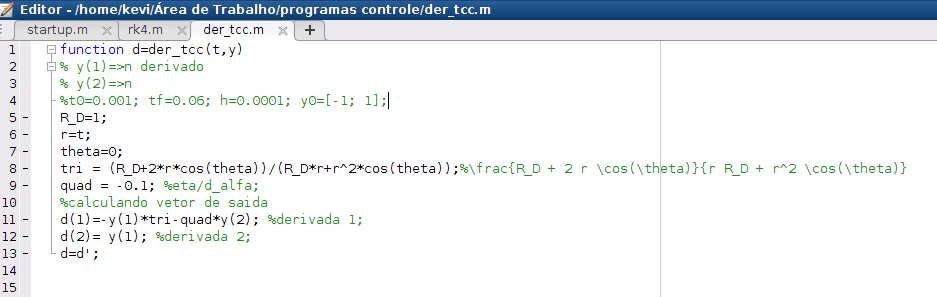
\includegraphics[scale=0.4]{exeplo.png} 
\caption{Algoritimo para a resolução numérica via \textit{rk4} de \ref{eqexe} no Matlab}
\end{figure}

\begin{figure}[H]
\centering
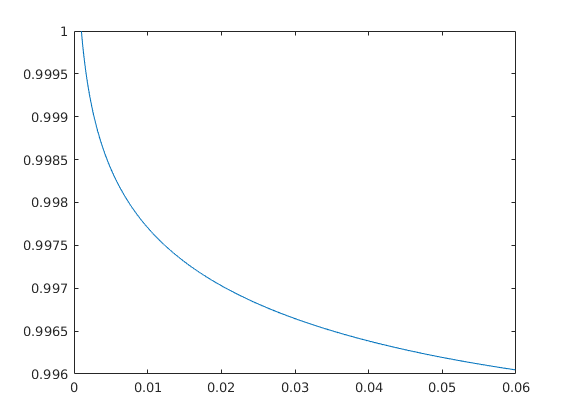
\includegraphics[scale=0.5]{exemplo1.png} 
\caption{Gráfico da resolução númerica de \ref{eqexe} no Matlab - Verticalmente temos o valor de $n(r)$ em $m^{-3}$, e horizontalmente o valor de $r$ em $m$.}
\end{figure}

Mudando as condições iniciais e o valor de $\frac{\eta}{D_\alpha}$ 

\begin{figure}[H]
\centering
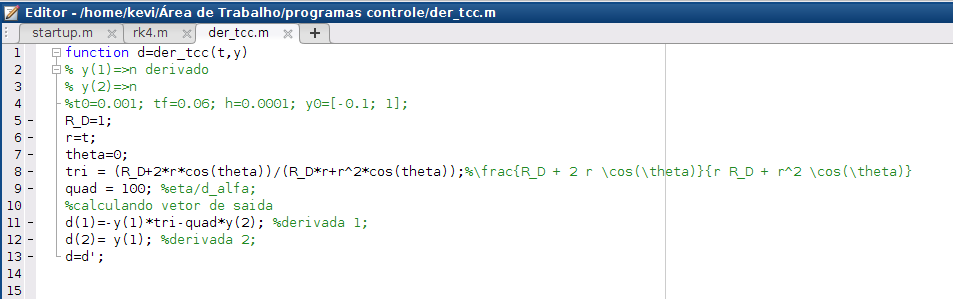
\includegraphics[scale=0.4]{exemplo2.png} 
\caption{Algoritimo para a resolução numérica via \textit{rk4} de \ref{eqexe} no Matlab}
\end{figure}

\begin{figure}[H]
\centering
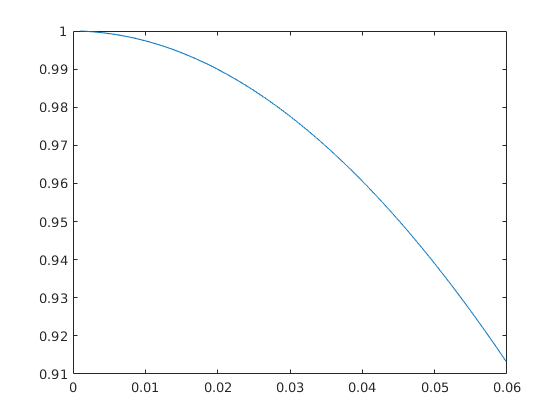
\includegraphics[scale=0.5]{exeplo2.png} 
\caption{Gráfico da resolução númerica de \ref{eqexe} no Matlab - Verticalmente temos o valor de $n(r)$ em $m^{-3}$, e horizontalmente o valor de $r$ em $m$.}
\end{figure}

\chapter{Fase Computacional}

Além dessas equações, devemos incluir equações para os campos eletromagnéticos. Vamos separar os campos em um componente gerado pelas correntes que fluem em bobinas fora do plasma e outro causado pelo plasma, ou seja, $\vv{E} = \vv{E}_{ext} + \vv{E}_{pl}$ e $\vv{B} = \vv{B}_{ext} + \vv{B}_{pl}$. O campo magnético aplicado externamente é produzido por um conjunto de bobinas específicas fora do plasma e possui componentes poloidais e toroidais. O campo toroidal tem uma dependência $1 / R$, enquanto o campo poloidal tem um padrão quadrupolo,
\begin{equation}
\vv{B}_{ext}=\vv{B}_{pol}^{quadrupole}+\frac{R_0B_0}{R\hat{e}_{\phi}}
\end{equation}
O campo elétrico aplicado externamente é produzido pelo solenóide central do tokamak, que induz uma voltagem de loop toroidal, $V_{loop}$. O campo elétrico externo é então dado por
\begin{equation}
\vv{E}_{ext} = \frac{V_{loop}}{2\pi R} \hat{e}_{\phi}
\end{equation}
O campo eletromagnético gerado pelo plasma é calculado via
\begin{equation}
\nabla A_{pl}=-u_0\vv{J}
\end{equation}
onde $A_{pl}$ é o vetor de potencial magnético devido ao plasma. O campo eletromagnético então segue de
\begin{equation}
B_{pl} = \nabla \times A_{pl}
\end{equation}

\begin{equation}
E_{pl}=-\frac{\partial A_{pl}}{\partial t}
\end{equation}

\section{Equipotenciais Campo Magnético}
Para obtermos as equipotenciais de campo magnético gerado pelas bobinas do tokamak Nova-Furg, é montado uma tabela de greem para o campo magnético gerado por cada bobina. Com uma corrente unitária, em uma \textit{mashgrid} que começa em 0.1 e vai até 0.73 no eixo horizontal e no vertical de -0.54 a 0.54. Tendo no seu centro o ponto central da seção reta do tokamak Nova-Furg.
Multiplicando então cada tabela de greem por uma corrente (Valores escolhidos apenas para obter uma distribuição, sem levar em conta os valores exatos reais), somando tudo e chamando a função \textit{contour} do Matlab obtemos a figura \ref{fig: equipotenc} onde temos as equipotenciais do campo magnético gerado pelas bobinas. E se adicionarmos o campo gerado pela corrente de plasma temos a figura \ref{fig: equipotenc2} onde temos as equipotenciais do campo magnético gerado pelas bobinas mais o campo magnético gerado pela corrente de plasma. No caso o o campo magnético gerado pela corrente de plasma é simulado por 5 bobinas localizadas no centro da secção reta do tokamak Nova-Furg.
\begin{figure}[H]
\centering
\caption{Equipotenciais Campo Magnético gerado pelas bobinas do Tokamak Nova-Furg - Imagem feita no Matlab, autoria própria}
\label{fig: equipotenc}
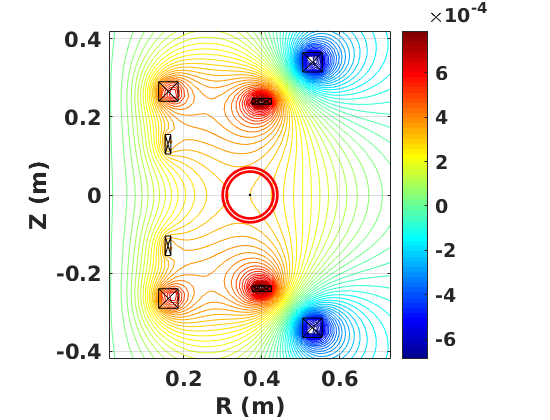
\includegraphics[scale=1.1]{../SImulacao_breakdown/Adaptacao_nova/campos_1.png} 
\end{figure}
Na figura \ref{fig: equipotenc} as correntes são: \\
Nas 2 bobinas de compensação externa 250 A.\\
Nas 2 bobinas de compensação interna 400 A.\\
Nas 2 bobinas verticais internas 1000A.\\ 
Nas 2 bobinas verticias externas 500A.\\
Na figura \ref{fig: equipotenc2} as correntes das bobinas são as mesmas só temos também a corrente de plasma total passando pelas 5 bobinas feitas para simualar a corrente de plasma que é -500 A.\\
A resoluão de \textit{mashgrid} usada é 65x65.
\begin{figure}[H]
\caption{Equipotenciais Campo Magnético  gerado pelas bobinas e corrente de plasma do Tokamak Nova-Furg - Imagem feita no Matlab, autoria própria}
\label{fig: equipotenc2}
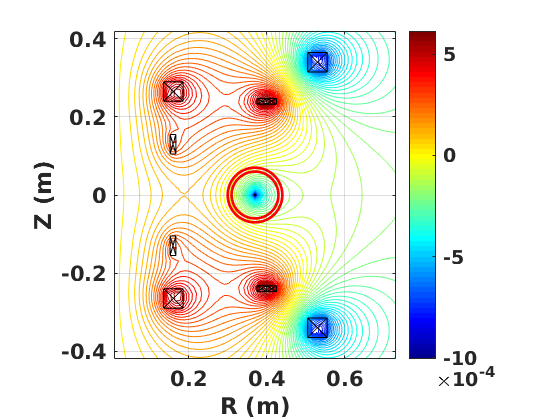
\includegraphics[scale=1.1]{../SImulacao_breakdown/Adaptacao_nova/campos_2.png} 
\end{figure}

\chapter{Resultados esperados}
Espero neste trabalho obter dados de simulação querentes com os medidos nos disparos do tokamak, para reforçar a válidade do modelo de dois fluidos para o \textit{breakdown}. Podendo então usar o modelo de dois fluidos para prever os resultados de cada experiemento na maquina. E se possível calcular quais os melhores parâmetros para operar o tokamak Nova-Furg.

\chapter{Conclusão}
Como resultados da fase teórica, logo no ínicio do trabalho vimos que existe claras diferenças entre os modelos de fluidos para o plasma e os modelos cinéticos. Também concluimos que para o nosso caso a melhor opção são os modelos de fluidos. Constatamos que a equação de Vlasov, Eq. \ref{eq: vlasov}, não é tão restritiva quanto parece uma vez que uma parte muito siguinificativa das interações entre partículas são consideradas nos campos elétromagneticos  internos suavizados $\vv{E}_i$ e $\vv{B}_i$ causados pela presença e movimento de todas as partículas carregadas dentro do plasma. Outro importante resultado obtido neste trabalho é o conjunto das 6 equações \ref{eq: pit51} de conservação dos momentos da equação de Boltzmann Eq. \ref{eq: boltsmam}, para cada momento são duas equações, uma para o fluido de elétrons e outra para o fluido de íons. Mas como vimos nas simplificações os íons podem ser considerados em repouso durante a fase inicial ou seja $\vv{u}_i = 0$, então pode-se remover a equação de conservação do momento iônico na faze de brackdown. Uma vez que a massa dos íons é muito maior que a massa dos elétrons implicando em uma mobilidade de íons muito menor. 
%\newpage
\appendix  
\chapter{O modelo de Townsend}
\label{Townsend}
O modelo de Townsend assume que os campos elétricos acionados externamente são predominantes no dispositivo. Tal suposição é verdadeira para dispositivos com gás neutro de baixa pressão e curto espaço entre os eletrodos, porque a quantidade de carga espacial local produzida durante o inicio do avalanche de elétrons é desprezível devido à pequena taxa de crescimento, $\alpha_T$. Portanto as características da avalanche de elétrons em dispositivos de baixa pressão de gás dependendem dos campos elétricos externos e podem ser descritas pelo modelo de Townsend. 

Assumindo que, devido à sua maior massa, os íons são estacionários, e os elétrons livres são responsáveis pela ionização.  O aumento da densidade eletrônica, $n_e$, é proporcional à diferença entre a taxa de ionização, $\nu_{ionz}$ (geração de elétrons) e a taxa de perda de elétrons, $\nu_{loss}$
\begin{equation}
\dfrac{dn_e}{dt} = (\nu_{ionz}-\nu_{loss})n_e
\label{cac0}
\end{equation}
portanto, nesta fase, a densidade eletronica $n_e(t)$ pode ser expressa como
\begin{equation}
n_e(t) = n_{e0} e^{(\nu_{ionz}-\nu_{loss})t}
\label{cac1}
\end{equation}
onde $t$ descreve o tempo, $n_{e0}$ é a densidade de elétrons em $t=0$ o \textit{breakdown} ocorre quando a taxa de geração de elétrons excede a taxa de perda de elétrons. Estes elétrons então são acelerados pelo campo elétrico toroidal e alcançam a velocidade de desvio (\textit{drift velocity}). Observe que a Eq. \ref{cac1} é válida somente quando o grau de ionização permanece pequeno, deste modo as colisões de elétrons com as partículas neutras predominam sobre as colisões Coulombianas. Para modelar o processo de ionização, vamos escrever a taxa de ionização em termos do primeiro coeficiente de Townsend e a velocidade de desvio do elétron 
\begin{equation}
\nu_{ionz} = \alpha_T u_{D,||}
\end{equation} 
onde $u_{D, ||}$ é a velocidade de desvio, $\alpha_T$ é o primeiro coeficiente de Townsend que é dado por
\begin{equation}
\alpha_T = A p_n e^{B \frac{p_n}{E_\Theta}}
\end{equation}

Aqui, $A$ e $B$ são constantes que dependem do gás de trabalho, $p_n$ é a pressão de gás neutro e  $E_\Theta$ é a magnitude do campo elétrio externo. A taxa de perda de elétrons devido ao seu movimento ao longo das linhas do campo magnético pode ser expressa por
\begin{equation}
\nu_{loss} = \frac{u_{D,||}}{L_{eff}}
\end{equation}
onde $L_{eff}$ é a distância média percorida pelo elétron antes de se chocar com a parede. Fazendo o lado direito da Eq. \ref{cac0} ir para zero, cria-se uma condição para o início do \textit{breakdown}
\begin{equation}
A p_n e^{B \frac{p_n}{E_\Theta}} = \frac{1}{L_{eff}}
\end{equation}
Esta equação mostra que um \textit{breakdown} bem-sucedido em um tokamak depende da escolha da pressão do gás neutro, da intensidade do campo elétrico toroidal e do comprimento efetivo da conexão ($L_{eff}$), que depende da configuração do campo poloidal durante a fase de partida. Existe então um valor mínimo do campo elétrico toroidal induzido para uma dada pressão de gás neutro e $L_{eff}$ para que se possa obter um \textit{breakdown}. Uma explicação detalhada para a modelagem da teoria de Townsend pode ser encontrada em \cite{yoo2014ohmic}
 



\chapter{Momentos da distribuição}
 Seja $\chi(v)$ uma propriedade física das partículas no plasma. Agora multiplicamos cada termo da Eq. \ref{eq: vlasov} por $\chi(v)$ e integramos a equação resultante sobre todo o espaço de velocidade para obter a equação como segue:

\begin{equation}
\label{eq: pit3}
\int_V \chi \frac{\partial f_\alpha}{\partial t} d^3 v + \int_V \chi \vv{v} \cdot \nabla f_\alpha d^3 v + \int_V \chi \vv{a} \cdot \nabla_v f_\alpha d^3 v = \int_V \chi (\frac{\delta f_\alpha}{\delta t})_{coll} d^3 v
\end{equation}
Resolvendo cada integral separadamente,

\begin{equation}
\label{eq: pit4}
\int_V \chi \frac{\partial f_\alpha}{\partial t} d^3 v  = \frac{\partial }{\partial t} (\int_V \chi f_\alpha d^3 v)-\int_V \frac{\partial \chi}{\partial t} f_\alpha d^3 v
\end{equation}
No entanto, desde que $\chi = \chi(\vv{v})$, sua derivada parcial em relação ao tempo é zero. Usando a definição de valores médios (Anexo. \ref{anexo1}), o rendimento fica
\begin{equation}
\label{eq: pit5}
\int_V \chi \frac{\partial f_\alpha}{\partial t} d^3 v = \frac{\partial}{\partial t} [n_\alpha(\vv{r},t)<\chi>_\alpha]
\end{equation}

\begin{equation}
\label{eq: pit6}
\int_V \chi \vv{v} \nabla f_\alpha d^3 v = \nabla \cdot \left( \int_V \chi \vv{v} f_\alpha d^3 v \right) - \int_V \nabla \chi \cdot \vv{v} f_\alpha d^3 v - \int_V \chi  f_\alpha \nabla \cdot \vv{v}  d^3 v
\end{equation}
Como visto anteriormente, $\chi = \chi(\vv{v})$, então seu gradiente é zero e as variáveis $\vv{r}$, $\vv{v}$ e $t$ são independentes, então o divergente de $\vv{v}$ também é zero, resultando em

\begin{equation}
\label{eq: pit7}
\int_V \chi \vv{v} \cdot \nabla f_\alpha d^3 v = \nabla \cdot [n_\alpha(\vv{r},t)<\chi \vv{v}>_\alpha]
\end{equation}

\begin{equation}
\label{eq: pit8}
\int_V \chi \vv{a} \cdot \nabla_v f_\alpha d^3 v = \int_V \nabla_v \cdot (\vv{a} \chi f_\alpha)d^3 v - \int_V f_\alpha (\vv{a} \cdot \nabla_v \chi) d^3 v - \int_V \chi  f_\alpha (\nabla_v \cdot \vv{a})  d^3 v
\end{equation}
A primeira integral desaparece porque a função de distribuição deve desaparecer para $\pm \infty$. A última integral na Eq. \ref{eq: pit8} desaparece se assumirmos que

\begin{equation}
\label{eq: pit9}
\nabla_v \cdot \vv{a} = \frac{1}{m_\alpha} \nabla_v \cdot \vv{F} = 0
\end{equation}
isto é, se o componente de força $F_j$ for independente do componente de velocidade correspondente $v_j$, uma vez que $\nabla_v \cdot \vv{F} = \sum_j \frac{\partial F_j}{\partial v_j}$. Isto é verdade para a força devido a um campo magnético, $\vv{F} = q_\alpha \vv{v} \times \vv{B}$ porque $j$ também neste caso $F_j$ é independente de $v_i$.

\begin{equation}
\label{eq: pit10}
\int_V \chi \vv{a} \cdot \nabla_v f_\alpha d^3 v = -n_\alpha(\vv{r},t)<\vv{a} \cdot \nabla_v \chi>_\alpha
\end{equation}

\begin{equation}
\label{eq: pit11}
\int_V \chi \left( \frac{\delta f_\alpha}{\delta t} \right)_{coll} d^3 v = \left[\frac{\delta}{\delta t}(n_\alpha(\vv{r},t)<\chi>_\alpha)\right]
\end{equation}

Combinando as Eq. \ref{eq: pit5}, Eq. \ref{eq: pit7}, Eq. \ref{eq: pit10} e Eq. \ref{eq: pit11} na Eq. \ref{eq: pit3} produzimos então,
\begin{equation}
\label{eq: pit12}
\frac{\partial }{\partial t}(n_\alpha(\vv{r},t)<\chi>_\alpha) + \nabla \cdot (n_\alpha(\vv{r},t)<\chi \vv{v} >_\alpha) - n_\alpha(\vv{r},t)<\vv{a} \cdot \nabla_v \chi>_\alpha = 
\end{equation}
\begin{equation*}
=[\frac{\delta}{\delta t}(n_\alpha(\vv{r},t)<\chi>_\alpha)]
\end{equation*}

\chapter{Lista de Notações}
\label{Listanot}
Lista de notação:\\
$\vv{E}_i$ é o campo elétrico macroscópico interno\\
$\vv{B}_i$ é o campo magnético macroscópico interno\\
$\vv{B}(\vv{r})$ é o vetor campo magnético\\
$\vv{E}(\vv{r})$ é o campo elétrico\\
$\vv{J}(\vv{r},t)$ é vetor densidade de corrente\\
$\nu_{ionz}$ é a taxa de ionização\\
$\nu_{loss}$ é a taxa de perda de elétrons\\
$n_{\alpha} = \int{f_\alpha(\vv{r},\vv{v},t)}d\vv{v}$ densidade númerica da partícula do tipo $\alpha$\\
$\vv{u}_{\alpha} = \frac{1}{n(\vv{r},t)} \int_V{\vv{v} f_{\alpha}(\vv{r},\vv{v},t) d^3v}$ é a velocidade média das partículas em $v$\\
$n_i$ é a densidade númerica de íons\\
$n_e$ é a densidade númerica de elétrons\\
$m_\alpha$ massa do tipo de partícula $\alpha$\\
$\alpha_a$ é o 1º coeficiente de Townsend para o tipo de partícula $\alpha$ \\
$\tau_p$ é o tempo de confinamento da partícula\\
$f_\alpha(\vv{r},\vv{v},t)$ é a função distribuição de velocidades.\\
$\rho(\vv{r},t)$ é a densidade de carga\\
$Q_\alpha$ representa a taxa de mudança de densidade de energia devido ao espalhamento\\
$\mathcal{E}_\alpha$ é a produção de partículas de plasma\\
 $\mathbb{P}_\alpha = \rho_{m\alpha}<\vv{c}_\alpha \cdot \vv{c}_\alpha>$ é o tensor de pressão cinética\\ 
$\vv{q}_\alpha = \frac{1}{2} \rho_{m\alpha} <c^2_\alpha  \vv{c}_\alpha>$ é o fluxo de calor \\
$q_\alpha$ é carga da partícula do tipo $\alpha$ \\
$D_e$, $D_i$, $D$ sendo os coeficientes de difusão de partículas. \\
$p(\vv{r},t)$ é o escalar de pressão\\
$e$ é  carga elementar do eletron\\
$\eta$ sendo a resistividade paralela do Spitzer\\
$\vv{R}_\alpha$ termo de troca de momento\\
$R_\alpha$ denota a taxa de mudança de momento devido ao espalhamento\\
$\mathcal{R}_\alpha$ denota a taxa de mudança de momento devido à produção de partículas de plasma.
\\
Operadores diferenciais:
\begin{equation*}
\nabla = \hat{e}_x \frac{\partial}{\partial x} + \hat{e}_y \frac{\partial}{\partial y} + \hat{e}_z \frac{\partial}{\partial z}
\end{equation*}

\begin{equation*}
\nabla^2 = \hat{e}_x \frac{\partial^2}{\partial x^2} + \hat{e}_y \frac{\partial^2}{\partial y^2} + \hat{e}_z \frac{\partial^2}{\partial z^2}
\end{equation*}

\begin{equation*}
\nabla_v = \hat{e}_x \frac{\partial}{\partial v_x} + \hat{e}_y \frac{\partial}{\partial v_y} + \hat{e}_z \frac{\partial}{\partial v_z}
\end{equation*} 

\chapter{Valor Médio}
O símbolo $<$  $>_\alpha$ denota o valor médio com respeito ao espaço de velocidades para o tipo de párticula $\alpha$, o valor médio é independente de $\vv{v}$ mas é uma função de $\vv{r}$ e $t$.
\begin{equation}
<\chi(\vv{r},\vv{v},t)>_\alpha = \frac{1}{n_\alpha(\vv{r},t)} \int_V \chi(\vv{r},\vv{v},t) f_\alpha(\vv{r},\vv{v},t) d^3 v
\label{anexo1}
\end{equation}
onde $V$ representa o espaço de velocidade, ou seja, todas as velocidades possíveis para cada partícula, $n_\alpha(\vv{r},t)=\int_V{f_\alpha(\vv{r},\vv{v},t)}d\vv{v}$ e a densidade númerica de partículas do tipo $\alpha$ na posição $\vv{r}$ no tempos $t$ e $f_\alpha(\vv{r},\vv{v},t)$ é a função distribuição de velocidades para as partículas do tipo $\alpha$.
\newpage
\chapter{Tabela Parâmetros Bobinas Nova-Furg}
Na tabela \ref{tab-nova} temos: 
\begin{table}[h]
\begin{center}
	\caption{Dados Nova-Furg}\label{tab-nova}
	\begin{tabular}{|c | c | c | c  |c | c |}
		\hline
		 Bobina & $R_0$ & $Z_0$ & $dR$ & $dZ$ & $J$ \\
		\hline
		 B1 & $0.1610$ & $0.2650$ & $0.050$ & $0.050$ & $ x $ \\
		 		\hline
		 B2 & $0.1610$ & $-0.2650$ & $0.050$ & $0.050$ & $ x $ \\
		 		\hline
		 B3 & $0.5300$ & $0.3400$ & $0.050$ & $0.050$ & $ y $ \\
		 		\hline
		 B4 & $0.5300$ & $-0.3400$ & $0.050$ & $0.050$ & $ y$ \\    
		 		\hline
         B5 & $0.3875$ & $0.2400$ & $0.025$ & $0.015$ & $w$ \\    
         		\hline
         B6 & $0.3875$ & $-0.2400$ & $0.025$ & $0.015$ & $w$ \\
         		\hline
         B7 & $0.1600$ & $0.1300$ & $0.015$ & $0.050$ & $ w $ \\     
         		\hline
         B8 & $0.1600$ & $-0.1300$ & $0.015$ & $0.050$ & $ w $ \\         
         		\hline
         B9 & $0.4125$ & $0.2400$ & $0.025$ & $0.015$ & $ k $ \\         
         		\hline
         B10 & $0.4125$ & $-0.2400$ & $0.025$ & $0.015$ & $ k $ \\         
         		\hline
         B11 & $0.1610$ & $-0.3000$ & $0.050$ & $0.050$ & $ l $ \\         
         		\hline
         B12 & $0.1610$ & $-0.3000$ & $0.050$ & $0.050$ & $ l $ \\         
         		\hline         		         		         		         		
	\end{tabular}
\end{center}
\end{table}



\begin{itemize}
\item B1 e B2 sendo as bobinas verticais internas; 
\item B3 e B4 sendo as bobinas verticais externas;  
\item B5 e B6 sendo as bobinas de compensação externas-internas;
\item B7 e B8 as bobinas de compensação internas;
\item B9 e B10 - sendo as bobinas de compensação externas-externas;
\item B11 e B12 - sendo as bobinas de aquecimento ohminico;
\item $R_0$ - raio onde se encontra o centro de cada bobina; 
\item $Z_0$ - altura onde se encontra o centro da bobina; 
\item $dR$ e $dZ$ são respectivamente, a variação ao longo do eixo $R$ da largura e ao longo do eixo $Z$ da altura;
\item $J$ - corrente que passa pela bobina;
\item o raio interno da camera de vácuo é 6 centímetros;
\item $x,y,w,k,l$ são valores de corrente que podem ser controlados.
\end{itemize}
\newpage
\begin{figure}[h]
\centering
\caption{Bobinas Tokamak Nova-Furg - Modelo criado no Blender, autoria própria}
\label{fig: btokamak}
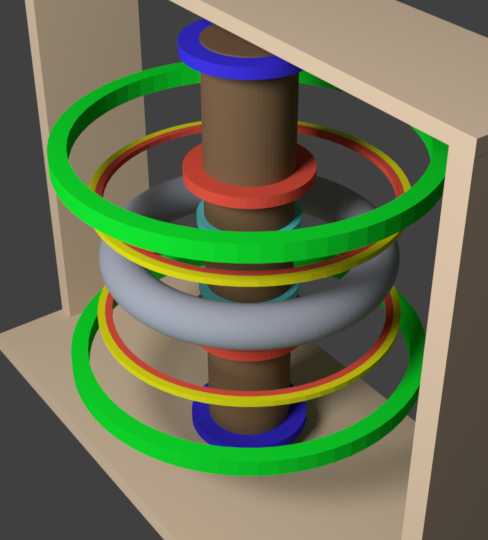
\includegraphics[scale=0.8]{bob2.png}  
\end{figure}
Na figura \ref{fig: btokamak} bobinas com mesma cor sempre possuem correntes iguais, onde temos de vermelho as duas bobinas verticais internas (B1 e B2) e as duas bobinas de compensação externas-internas (B5 e B6); de verde as duas bobinas verticais externas (B3 e B4); de azul claro as duas bobinas de compensação internas (B7 e B8); de amarelo as duas bobinas de compensação externas-externas (B9 e B10) e de azul as duas bobinas de aquecimento ohminico (B11 e B12);



\chapter{Tabela de Unidades Úteis}
A Tabela \ref{tabela1} apresenta algumas unidades úteis para este trabalho.
    
    \begin{table}[ht]
    \caption{Relação entre unidades}
    \label{tabela1}
    \begin{center}
    \begin{tabular}{lll}
    \hline 
    Unidade & Simbolo & Relações \\ 
    \hline 
    Metro & $m$  & $\left[ \frac{N \cdot s^2}{Kg} \right]$ \\ 
     \\
    Kilograma  & $Kg$ & $\left[ \frac{J \cdot s^2}{m^2} \right]$  \\ 
     \\
    Newton & $N$  & $\left[  \frac{kg \cdot m}{s^2}\right]$ \\ 
     \\   
    Segundo & $s$  & $\vv{v} = \left[ m/s \right]$ \\ 
     \\
    Ampere & $A$  & $\left[ \frac{C}{s}\right]$ \\ 
     \\
    Coulonb & $C$  & $\left[ A \cdot s = F \cdot V\right]$ \\ 
     \\
    Tesla & $T$  & $\left[ \frac{V \cdot s}{m^2} = \frac{N}{A \cdot m} = \frac{J}{A \cdot m^2} \right]$ \\ 
     \\
    Joule & $J$  & $\left[ \frac{kg \cdot m^2}{s^2} \right]$ \\ 
    \\
    Farad & $F$  & $\left[ \frac{C}{V} = \frac{A \cdot s}{V} = \frac{J}{V^2} = \frac{s}{\Omega} = \frac{s^2 \cdot C^2}{m^2 \cdot Kg} \right]$ \\ 
      \\  
    Watt & $W$  & $\left[ \frac{J}{s} = \frac{N \cdot m}{s} = \frac{Kg \cdot m^2}{s^3} \right]$ \\ 
    \\
    Volt & $V$  & $\left[ A \cdot \Omega = \frac{W}{A} = \frac{J}{C} = \frac{eV}{e}\right]$ \\ 
     \\
    eletro-Volt & $eV$  & $\left[ 1.6 \times 10^{-19}J \right]$ \\
    \\
    Ohn & $\Omega$  & $\left[ \frac{V}{A} = \frac{W}{A^2} = \frac{V^2}{W} = \frac{s}{F} \right]$ \\ 
  
      
    \hline
    
    \end{tabular}
    \end{center}         
    \end{table}
%\newpage
%\annex
    
\endgroup

%\newpage

\bibliography{TCC_1}






\end{document}
